\section{Process simulation}
\subsection{Process Simulation - 3}
From the implantation profile plot Fig.  \ref{fig:implantation_profile} and the .out files generated, the peak concentrations  for Sb is approximately $1.32904 \times 10^{20}\text{ cm}^{-3}$ at 0.086 µm, and for As, it is about $1.12664 \times 10^{20}\text{ cm}^{-3}$ at 0.091 µm, and the peak concentration of B  is roughly $1.00165 \times 10^{20}\text{ cm}^{-3}$ at 0.093 µm.
\begin{figure}[H]
    \centering
    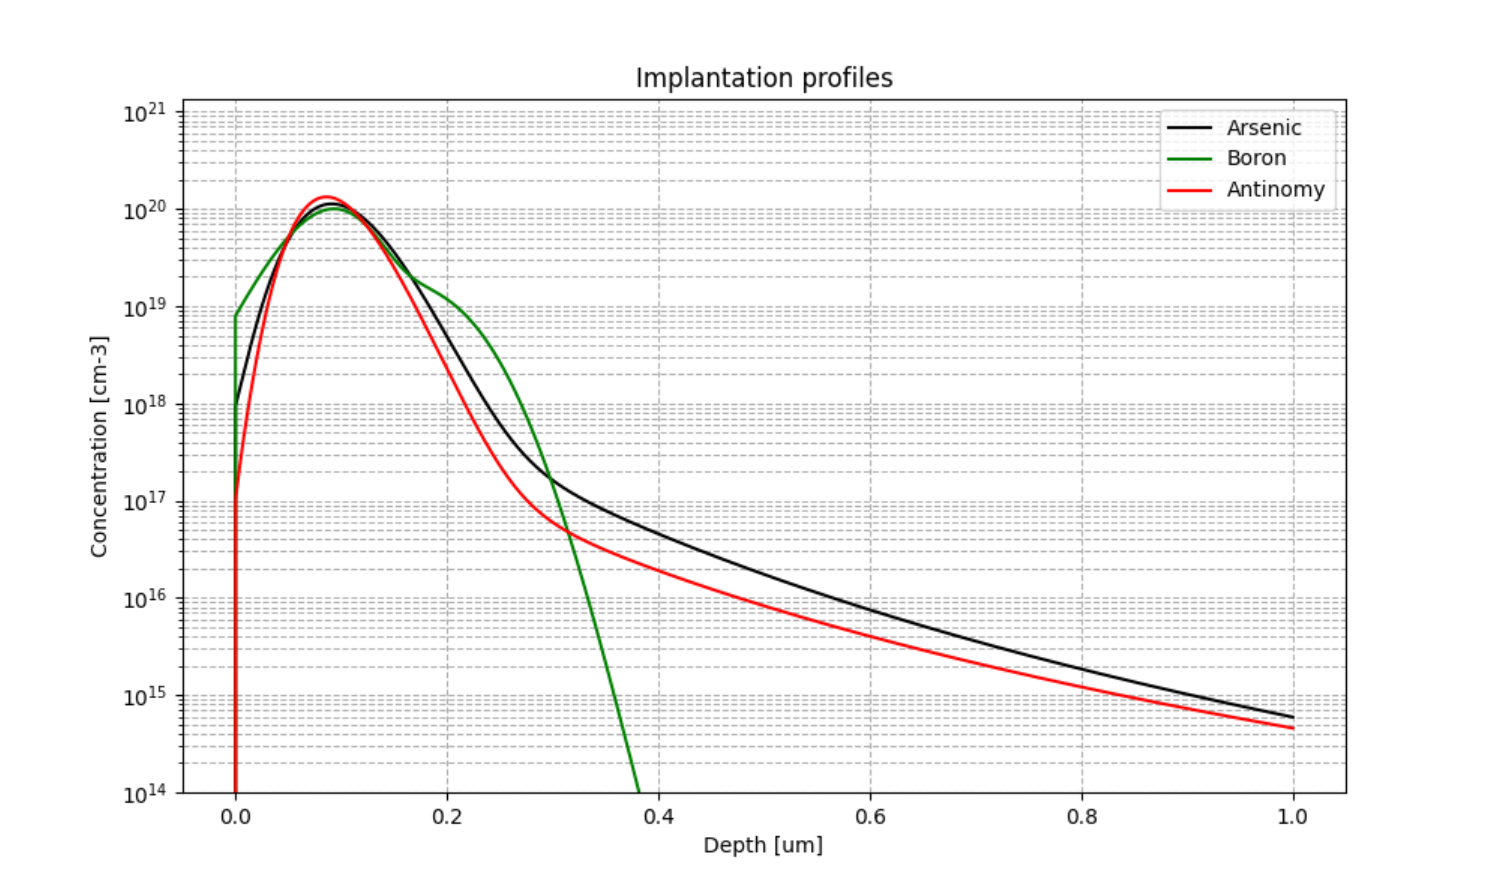
\includegraphics[width=0.7\linewidth]{Figures/implant_py.png}
    \caption{Simulated implantation profiles of arsenic (black), boron(green) and antimony (red) in crystalline silicon at matched projected range.}
    \label{fig:implantation_profile}
\end{figure}

 None of the profiles is Gaussian because standard Gaussian would appear as a symmetric, inverted parabola on a log plot. Among Boron, Arsenic and Antimony, Boron has the shortest tail because the profile drops below $10^{13} \text{ cm}^{-3}$ already at $0.4\text{ }\mu\text{m}$. Antimony has a longer tail than boron, but its concentration is lower than Arsenic at larger depths. Arsenic has the longest tail because its concentration is still above Antimony at the depth of 1 µm.

\subsection{Process Simulation - 4}
From \verb|implant-B.cmd|, \verb|implant-As.cmd|, \verb|implant-Sb.cmd|, the energy of B, As, and Sb are 24 keV, 148 keV and 200 keV respectively. As and Sb are As P lies between B and As, one way to estimate the energy of P used in implanation is using linear interpolation between B and As

\begin{gather*}
E_{P} = E_{B} + \frac{m_{P} - m_{B}}{m_{As} - m_{B}} (E_{As} - E_{B}) 
\end{gather*}
As the relative atomic mass of P, B and As are 31, 11 and 75 respectively, Substitution into the equation above gives
\begin{gather*}
E_{P} = 24 + \frac{31 - 11}{75 - 11} (148 - 24) = 24 + \frac{20}{64} \times 124 \approx 62.75 \text{ keV} 
\end{gather*}
Therefore, the energy used in \verb|implant-P.cmd| is selected as $E_{P} \approx 63 \text{ keV}$.

Setting \verb|energy=63| in \verb|implant-P.cmd| and rerunning the implant.py gives the plt shown in Fig. \ref{fig:implantation_profile_with_p}. The implantation profile of P is the blue curve.

From the generated .out file, the peak concentration of P, which is $1.19169 \times 10^{20}\text{ cm}^{-3}$, appears at the depth of 0.080 µm. The resulting implantation profile has its peak at approximately the same depth as the other three dopants (Sb at 0.086 µm, As at 0.091 µm, B at 0.093 µm), so this energy is a reasonable estimate.

\begin{figure}[H]
    \centering
    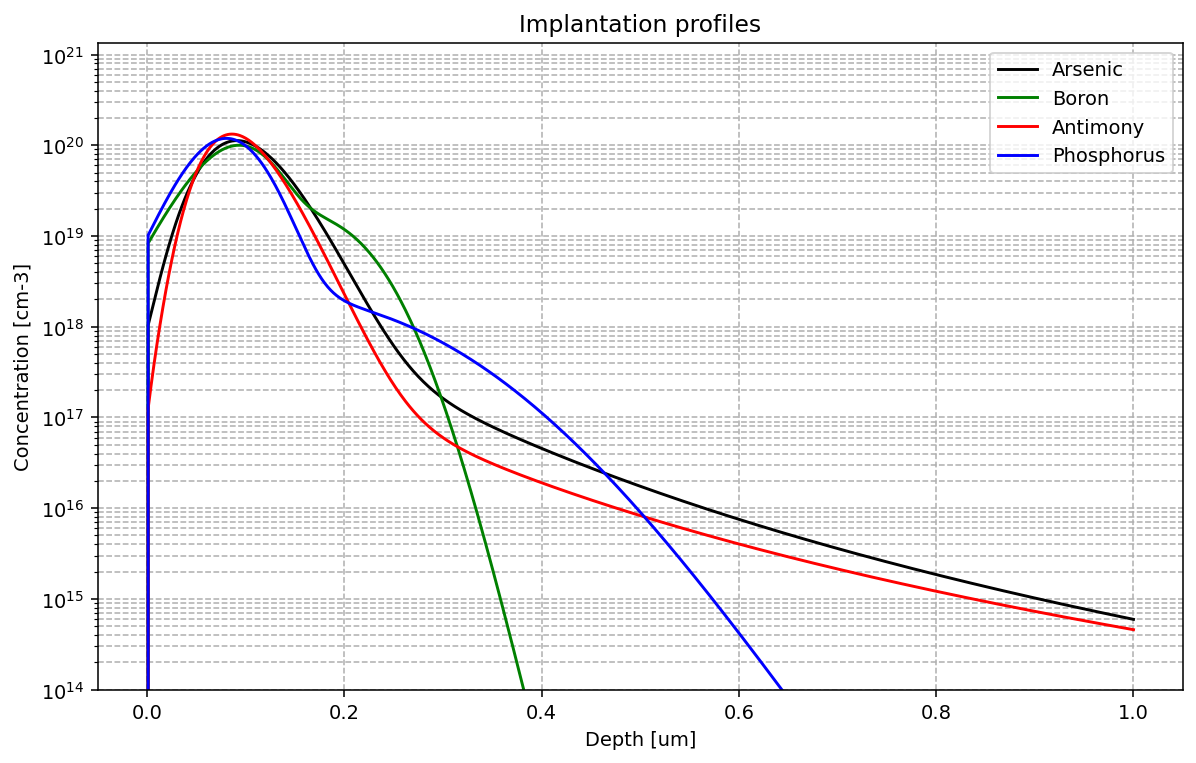
\includegraphics[width=0.7\linewidth]{Figures/implant_with_p_py.png}
    \caption{Simulated implantation profiles of arsenic (black), boron(green), phosphorous(blue), and antimony (red) in crystalline silicon at matched projected range.}
    \label{fig:implantation_profile_with_p}
\end{figure}


\subsection{Process Simulation - 5}
The implantation profiles of Boron, Phosphorus, Arsenic and Antimony in amorphous silicon are shown in Fig. \ref{fig:armorf_profile} below
\begin{figure}[H]
    \centering
    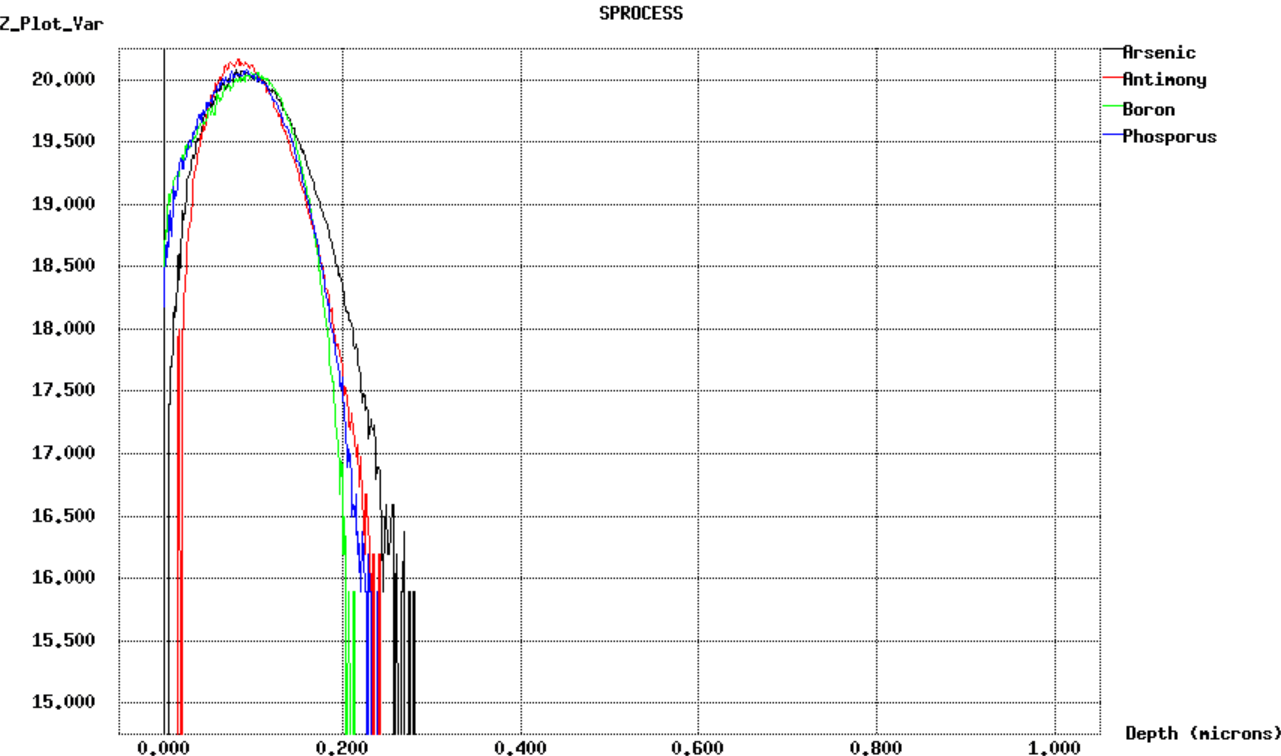
\includegraphics[width=0.75\linewidth]{Figures/armorf_cmd.png}
    \caption{Simulated implantation profiles in amorphous silicon}
    \label{fig:armorf_profile}
\end{figure}

In amorphous silicon, all implantation profiles are closer to a Gaussian distribution. This is because amorphous silicon has no crystal channels, so channeling is strongly reduced. The implantation ions cannot travel deeply along specific lattice directions.

All implantations can be run after each other in armorphous silicon because the substrate is amorphous. The damage caused by one implantation doesn't change the crystal channeling behaviour of the following implantation. 

In contrast, the implantations in crystalline silicon were simulated separately because the damage from one implantation could affect the next implantation.



\subsection{Process Simulation - 6 \& 7}
After running the script with the default setting, which is 40 keV and the tilt of the implantation is $7 \degree$, the plot generated is shown below.
\begin{figure}[H]
    \centering
    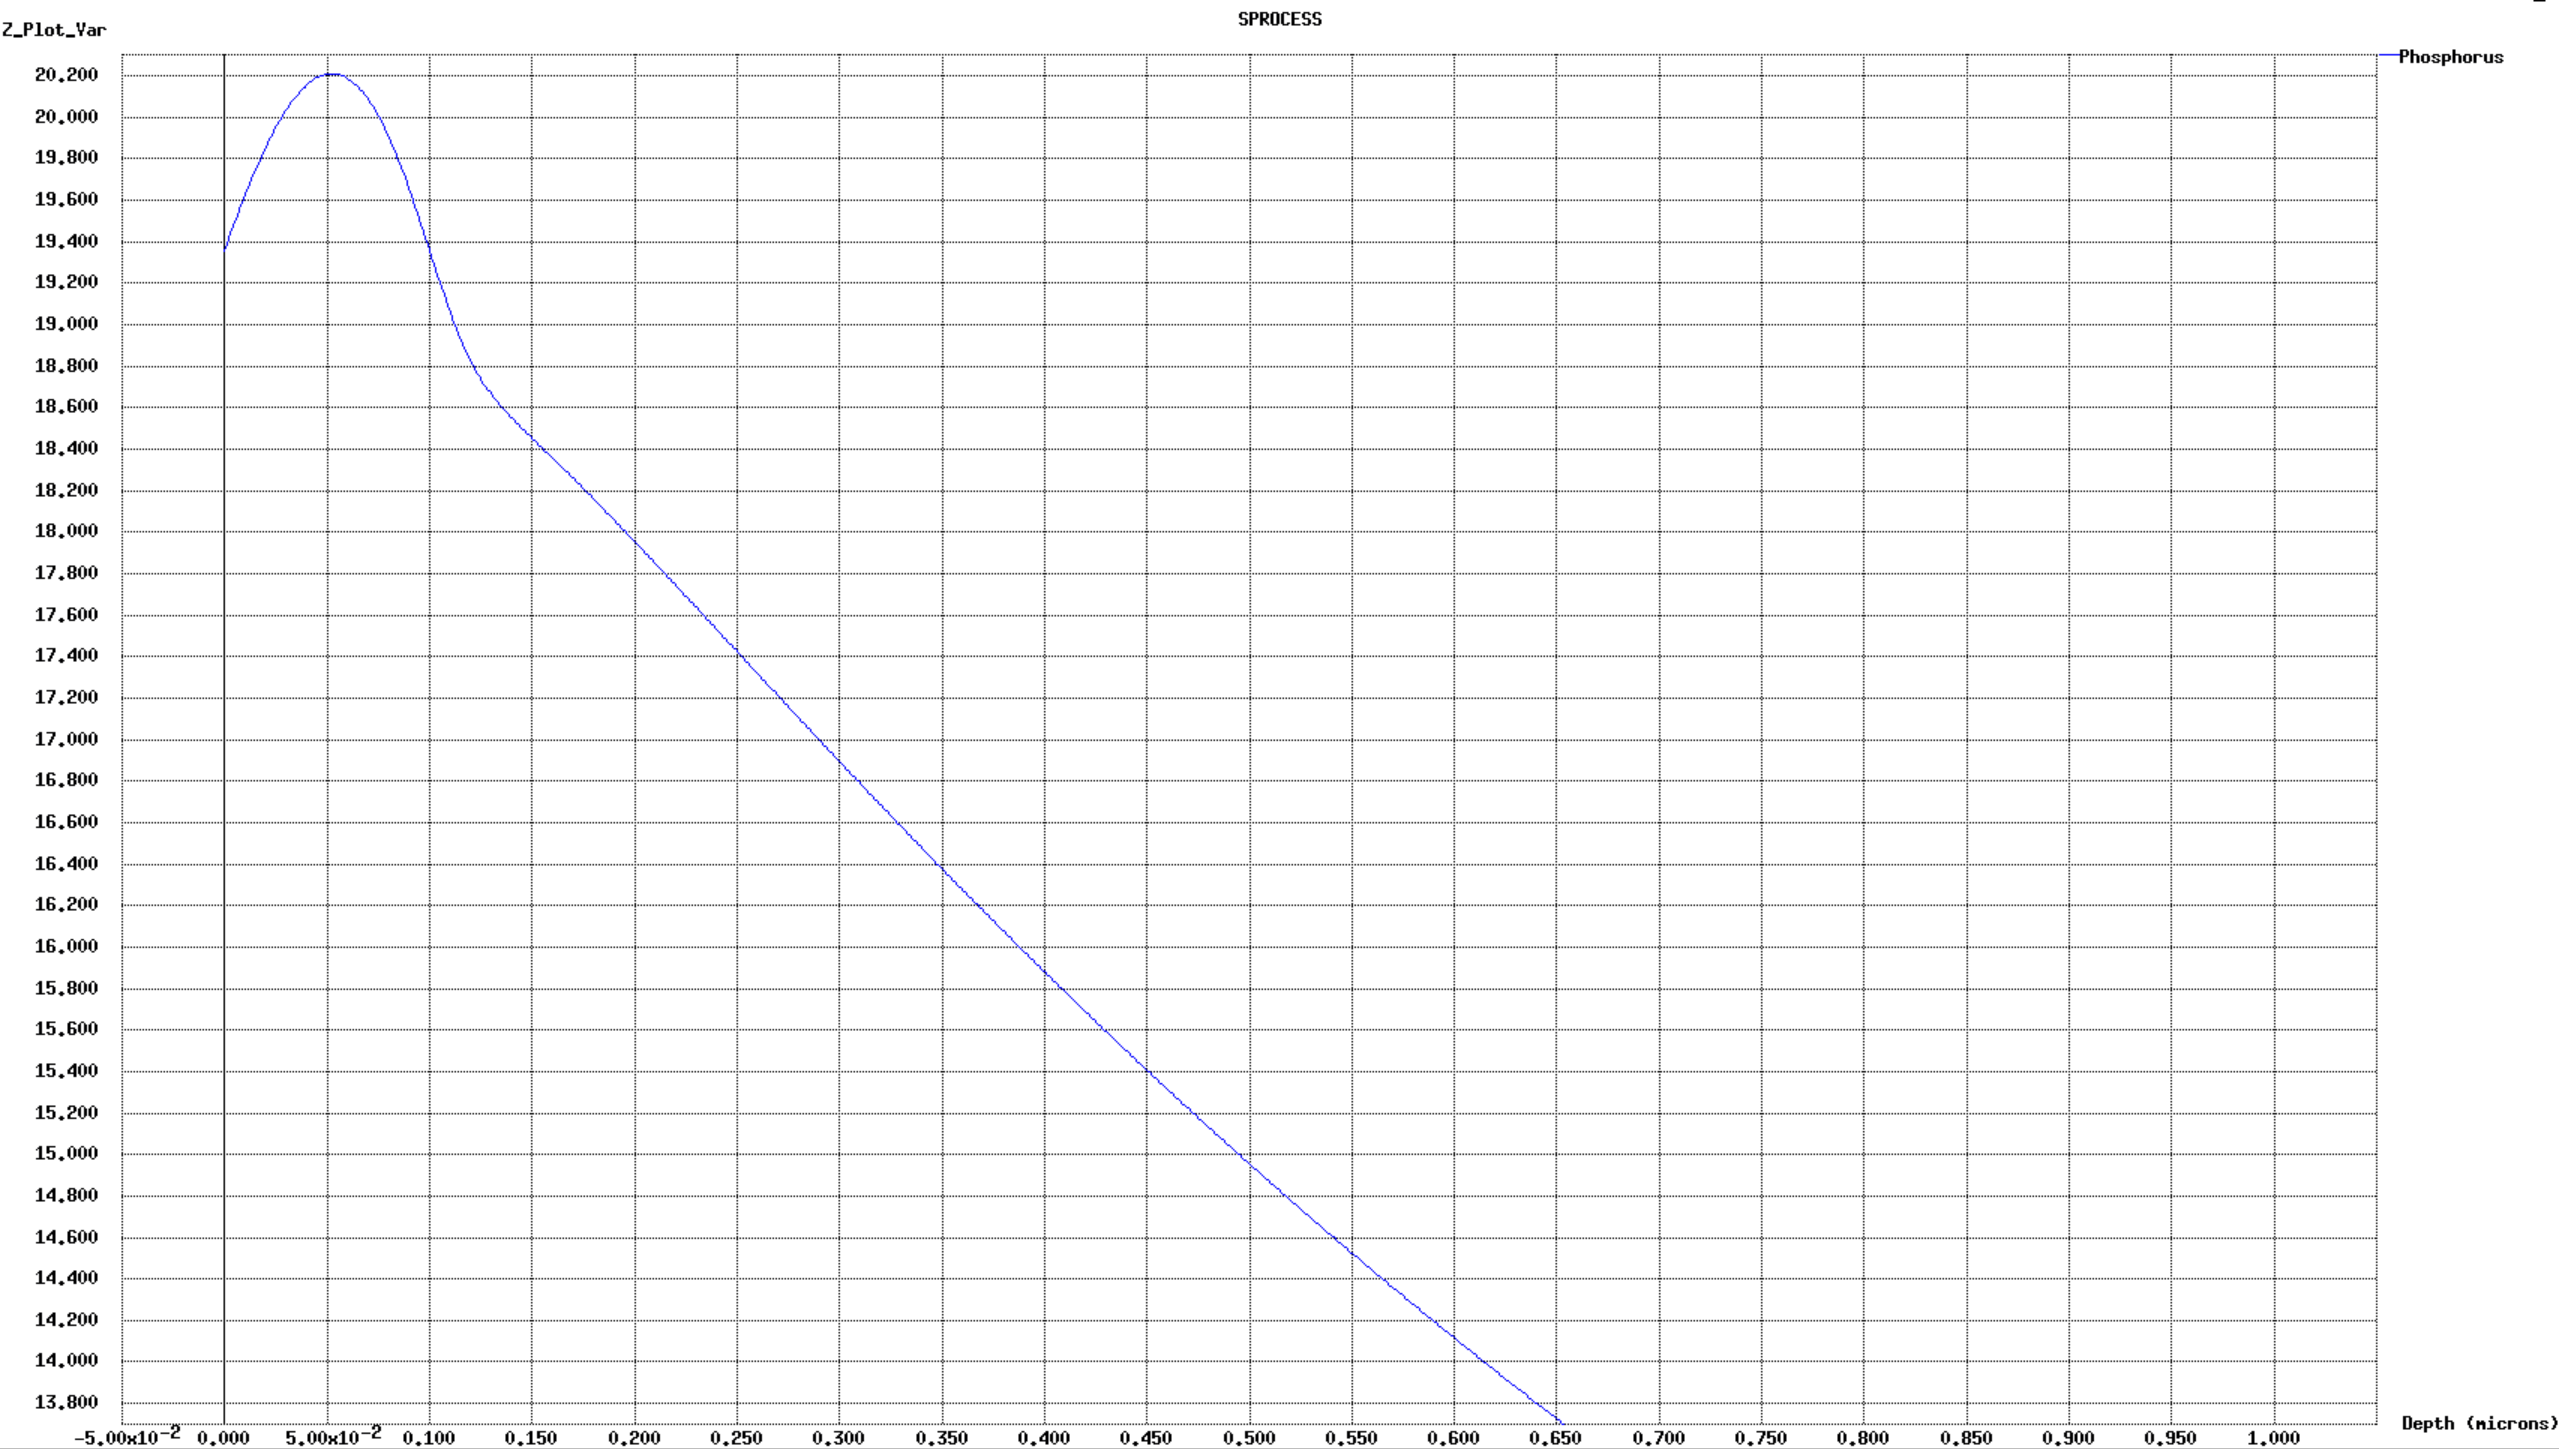
\includegraphics[width=0.7\linewidth]{Figures/tilt_7.png}
    \caption{Phosphorus implantation profiles with the energy of 40\,keV for tilt angle of 7\textdegree}
    \label{fig:tilt_7}
\end{figure}

Using the generated .out files, the implantation profiles of Phosphorus with 40 keV and 6 different tilt angles, including the default $7\degree$, $0\degree$, $3\degree$, $11\degree$, $13\degree$ and $15\degree$, are shown in Fig. \ref{fig:tilt_sweep}.
\begin{figure}[H]
    \centering
    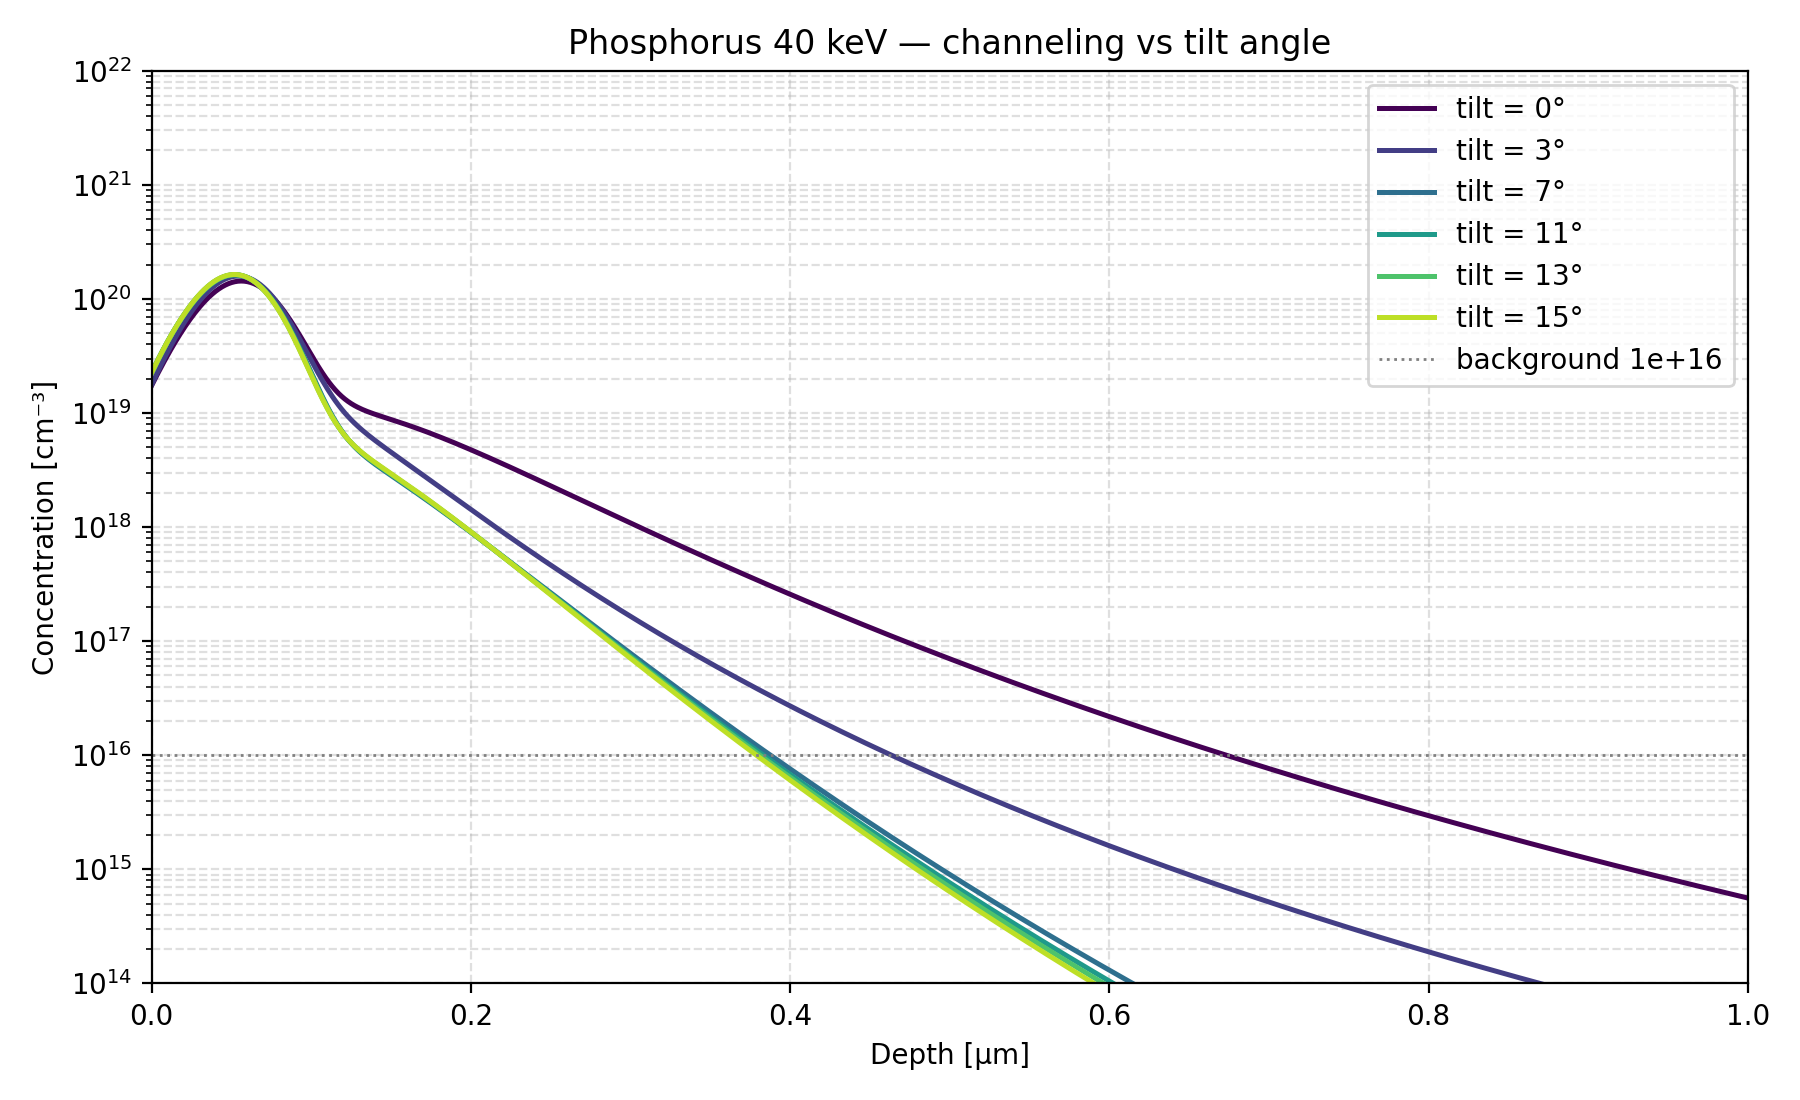
\includegraphics[width=0.75\linewidth]{Figures/tilt_sweep.png}
    \caption{Phosphorus implantation profiles with the energy of 40\,keV for tilt angles of 0\textdegree, 3\textdegree, 7\textdegree, 11\textdegree,13\textdegree and 15\textdegree}
    \label{fig:tilt_sweep}
\end{figure}

From the simulation results, $7\degree$ is the smallest tilt that is able to suppress the channeling tail, and larger tilt angles give no further improvement.



\subsection{Process Simulation - 8}
The dopant profiles after implantation in amorphous silicon followed by diffusion at $1000^\circ\mathrm{C}$ for 5 hours is shown in Figure~\ref{fig:diffamorf}.

\begin{figure}[H]
    \centering
    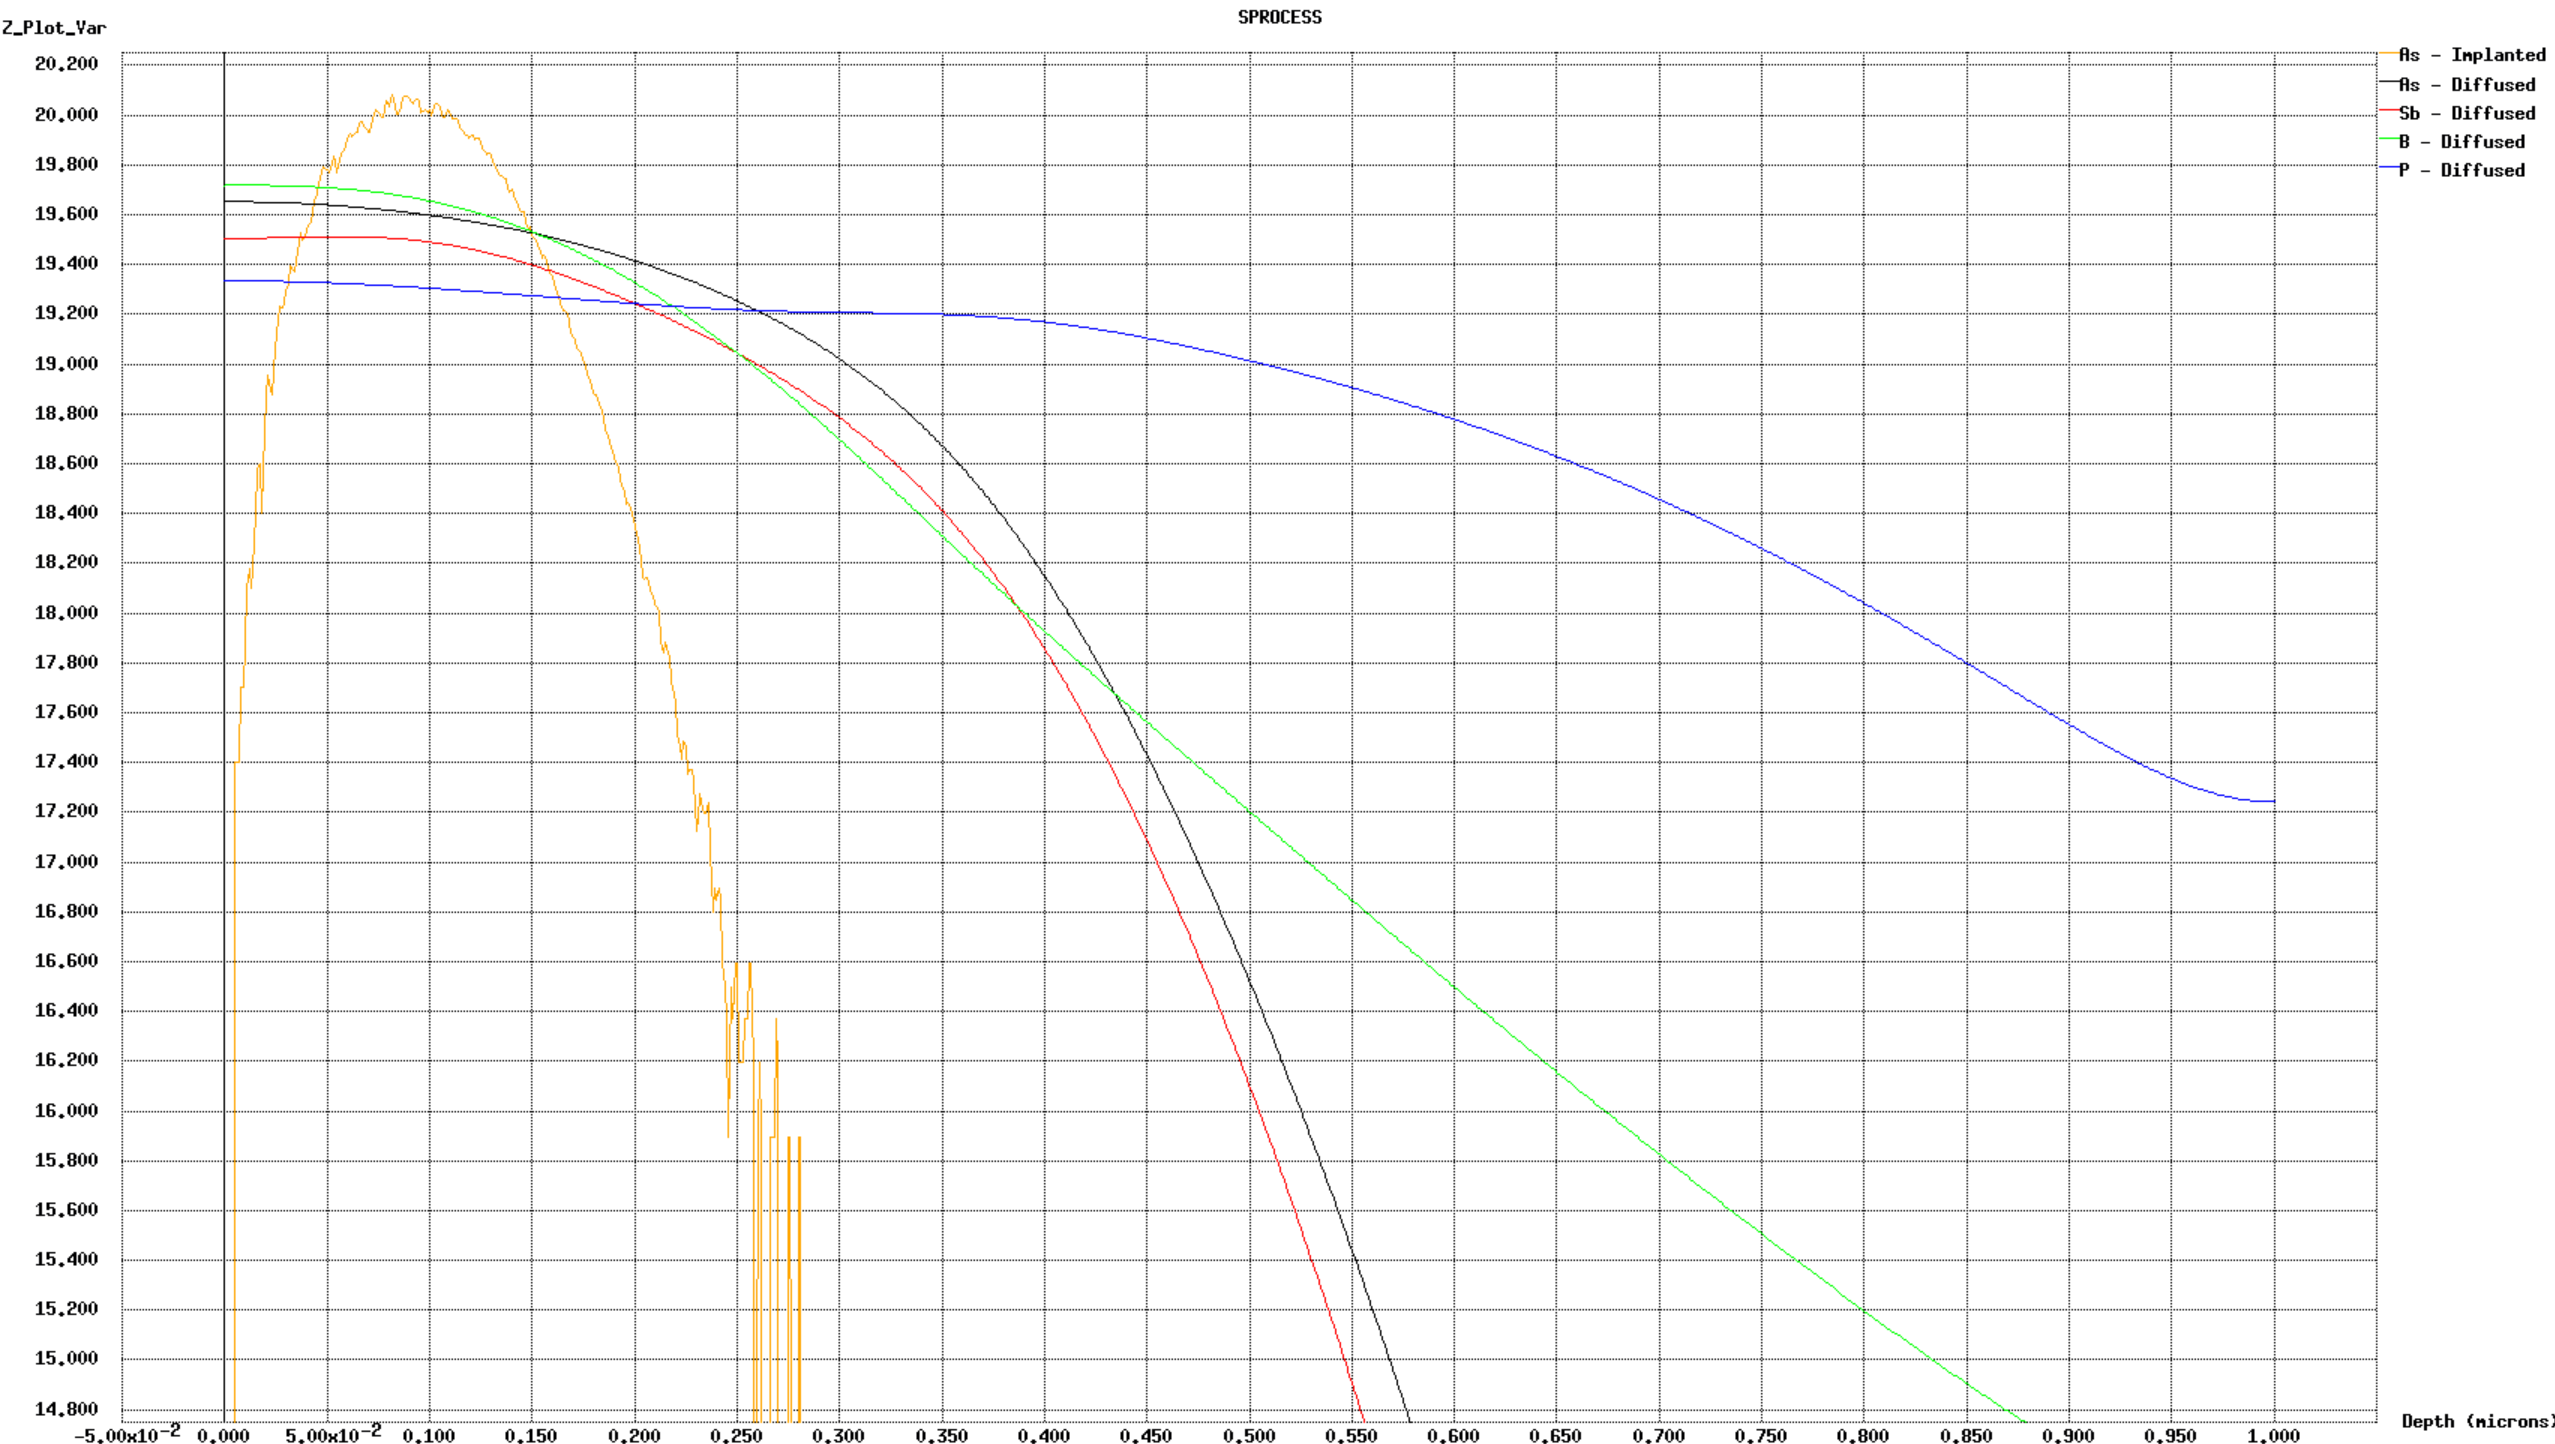
\includegraphics[width=0.7\linewidth]{Figures/diffamorf.png}
    \caption{Diffused dopant profiles after 5 hours at $1000^\circ\mathrm{C}$. The orange curve shows the implantation profile of As before diffusion.}
    \label{fig:diffamorf}
\end{figure}

From the simulated results, from narrowest to widest diffusion profile, the dopants can be ordered as

\[
\mathrm{Sb} < \mathrm{As} < \mathrm{B} < \mathrm{P}
\]

Antimony and arsenic are relatively narrow, while boron and especially phosphorus diffuse much further into the silicon. 

According to Table \ref{tab:misfit_factor}, dopants with negative misfit factors, e.g. boron and phosphorus, show
stronger diffusion, while dopants with no misfit (As) or with positive misfit (Sb) diffuse less.
\begin{table}[h]
    \centering
    \caption{Solid solubility limit and misfit factor for different dopants.}
    \label{tab:misfit_factor}
    \begin{tabular}{lcccc}
        \toprule
        Dopant & Solid solubility limit (cm$^{-3}$) & Max active dopants (cm$^{-3}$) & Radius (\AA) & Misfit factor \\
        \midrule
        B  & $4 \times 10^{20}$   & $5 \times 10^{19}$ & 0.88 & $-0.254$ \\
        P  & $1.5 \times 10^{21}$ & $1 \times 10^{21}$ & 1.10 & $-0.068$ \\
        As & $2 \times 10^{21}$   & $2 \times 10^{21}$ & 1.18 & $0$      \\
        Sb & $1 \times 10^{20}$   & $2 \times 10^{19}$ & 1.36 & $+0.153$ \\
        \bottomrule
    \end{tabular}
\end{table}

 Therefore, the simulation shows a relation between misfit factor and diffusion width, although the relation between the misfit factor and diffusion width is clearly not proportional.

 \subsection{Process Simulation - 9}
The implantation and diffusion profiles of Sb for two different implantation doses ($1\times10^{15}~\mathrm{cm^{-2}}$ and 
$1\times10^{14}~\mathrm{cm^{-2}}$) are plotted.

For the default dose (Fig.~\ref{fig:impl_1e15}), the implanted peak reaches $1.32843 \times 10^{20}$ cm$^{-3}$, which is above the Sb solid solubility limit at 1150\,\textdegree C ($1 \times 10^{20}$ cm$^{-3}$). After diffusion, the profile near the peak takes a hat-like shape. The excess Sb above the limit cannot occupy lattice sites and forms inactive clusters, so the active concentration is held at the cap until the profile falls below the solubility limit.

\begin{figure}[H]
    \centering
    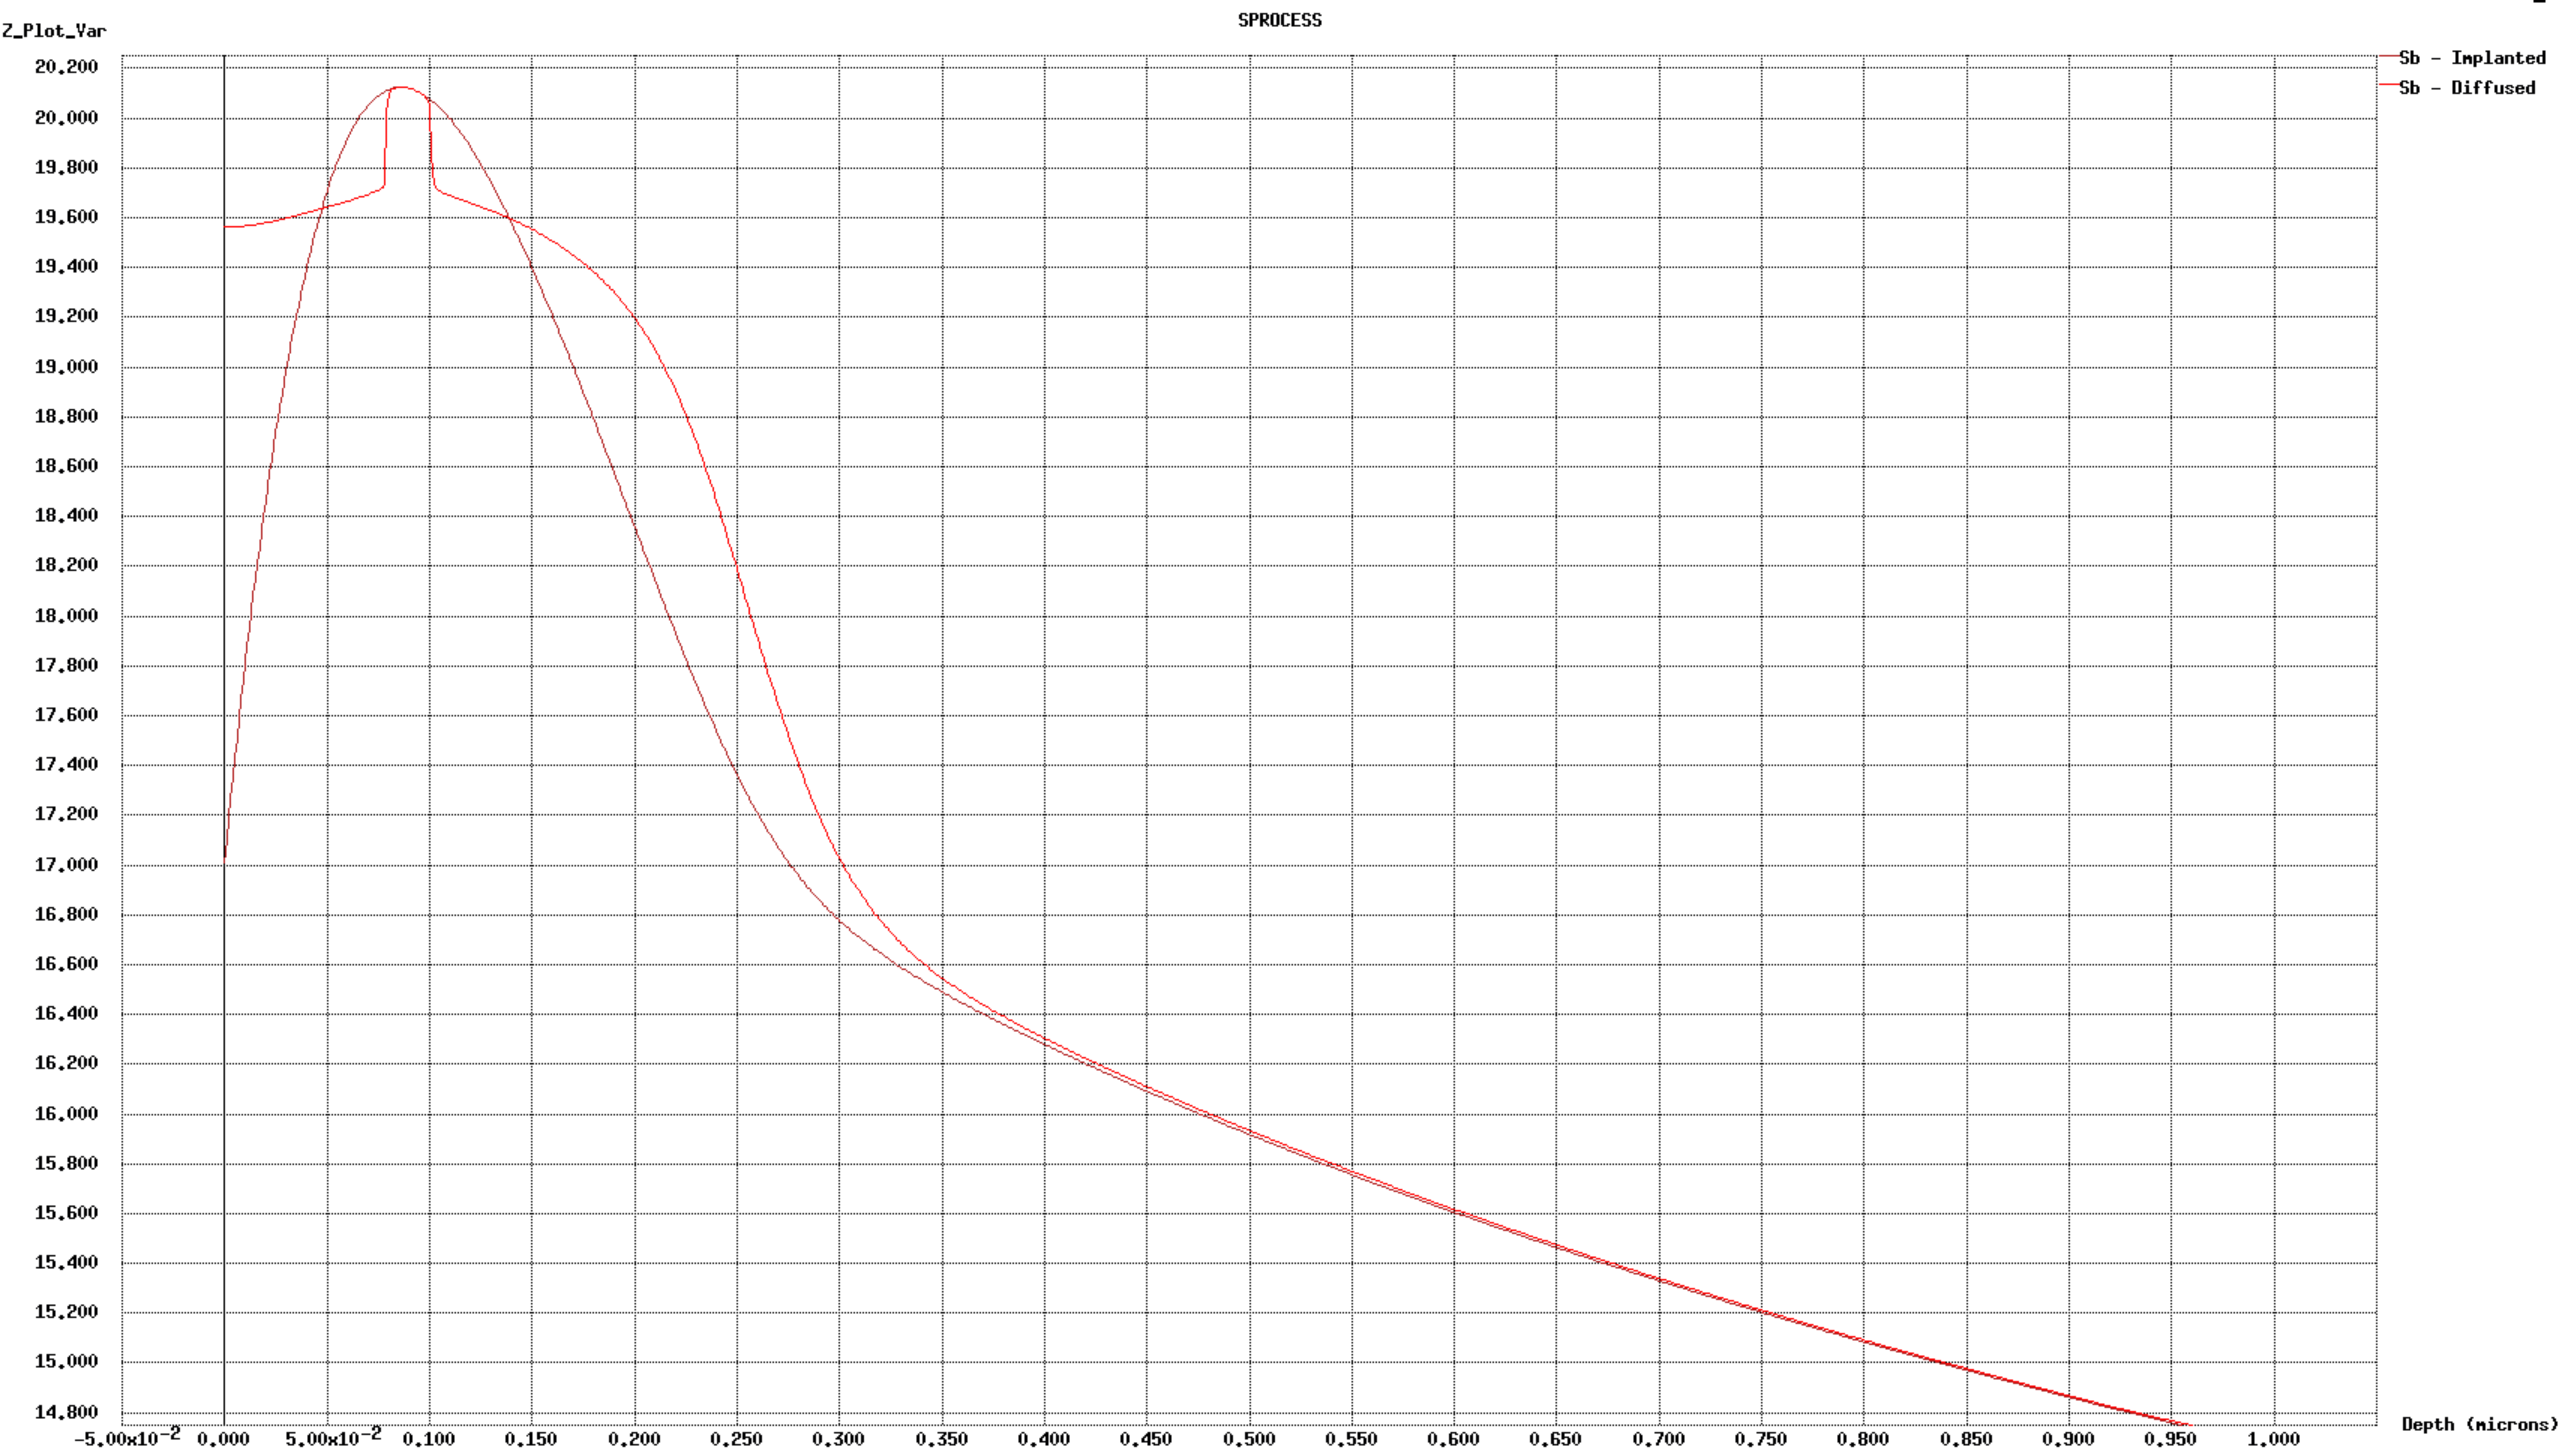
\includegraphics[width=0.7\linewidth]{Figures/impl_1e15.png}
    \caption{Antimony implantation and diffusion profile for a dose of
    $1\times10^{15}~\mathrm{cm^{-2}}$.}
    \label{fig:impl_1e15}
\end{figure}

For the reduced dose (Fig. \ref{fig:impl_1e14}), the peak of implantation profile is $7.79507 \times 10^{18}$ cm$^{-3}$, which is below the solubility limit. and
the diffused profile is therefore smoother.

\begin{figure}[H]
    \centering
    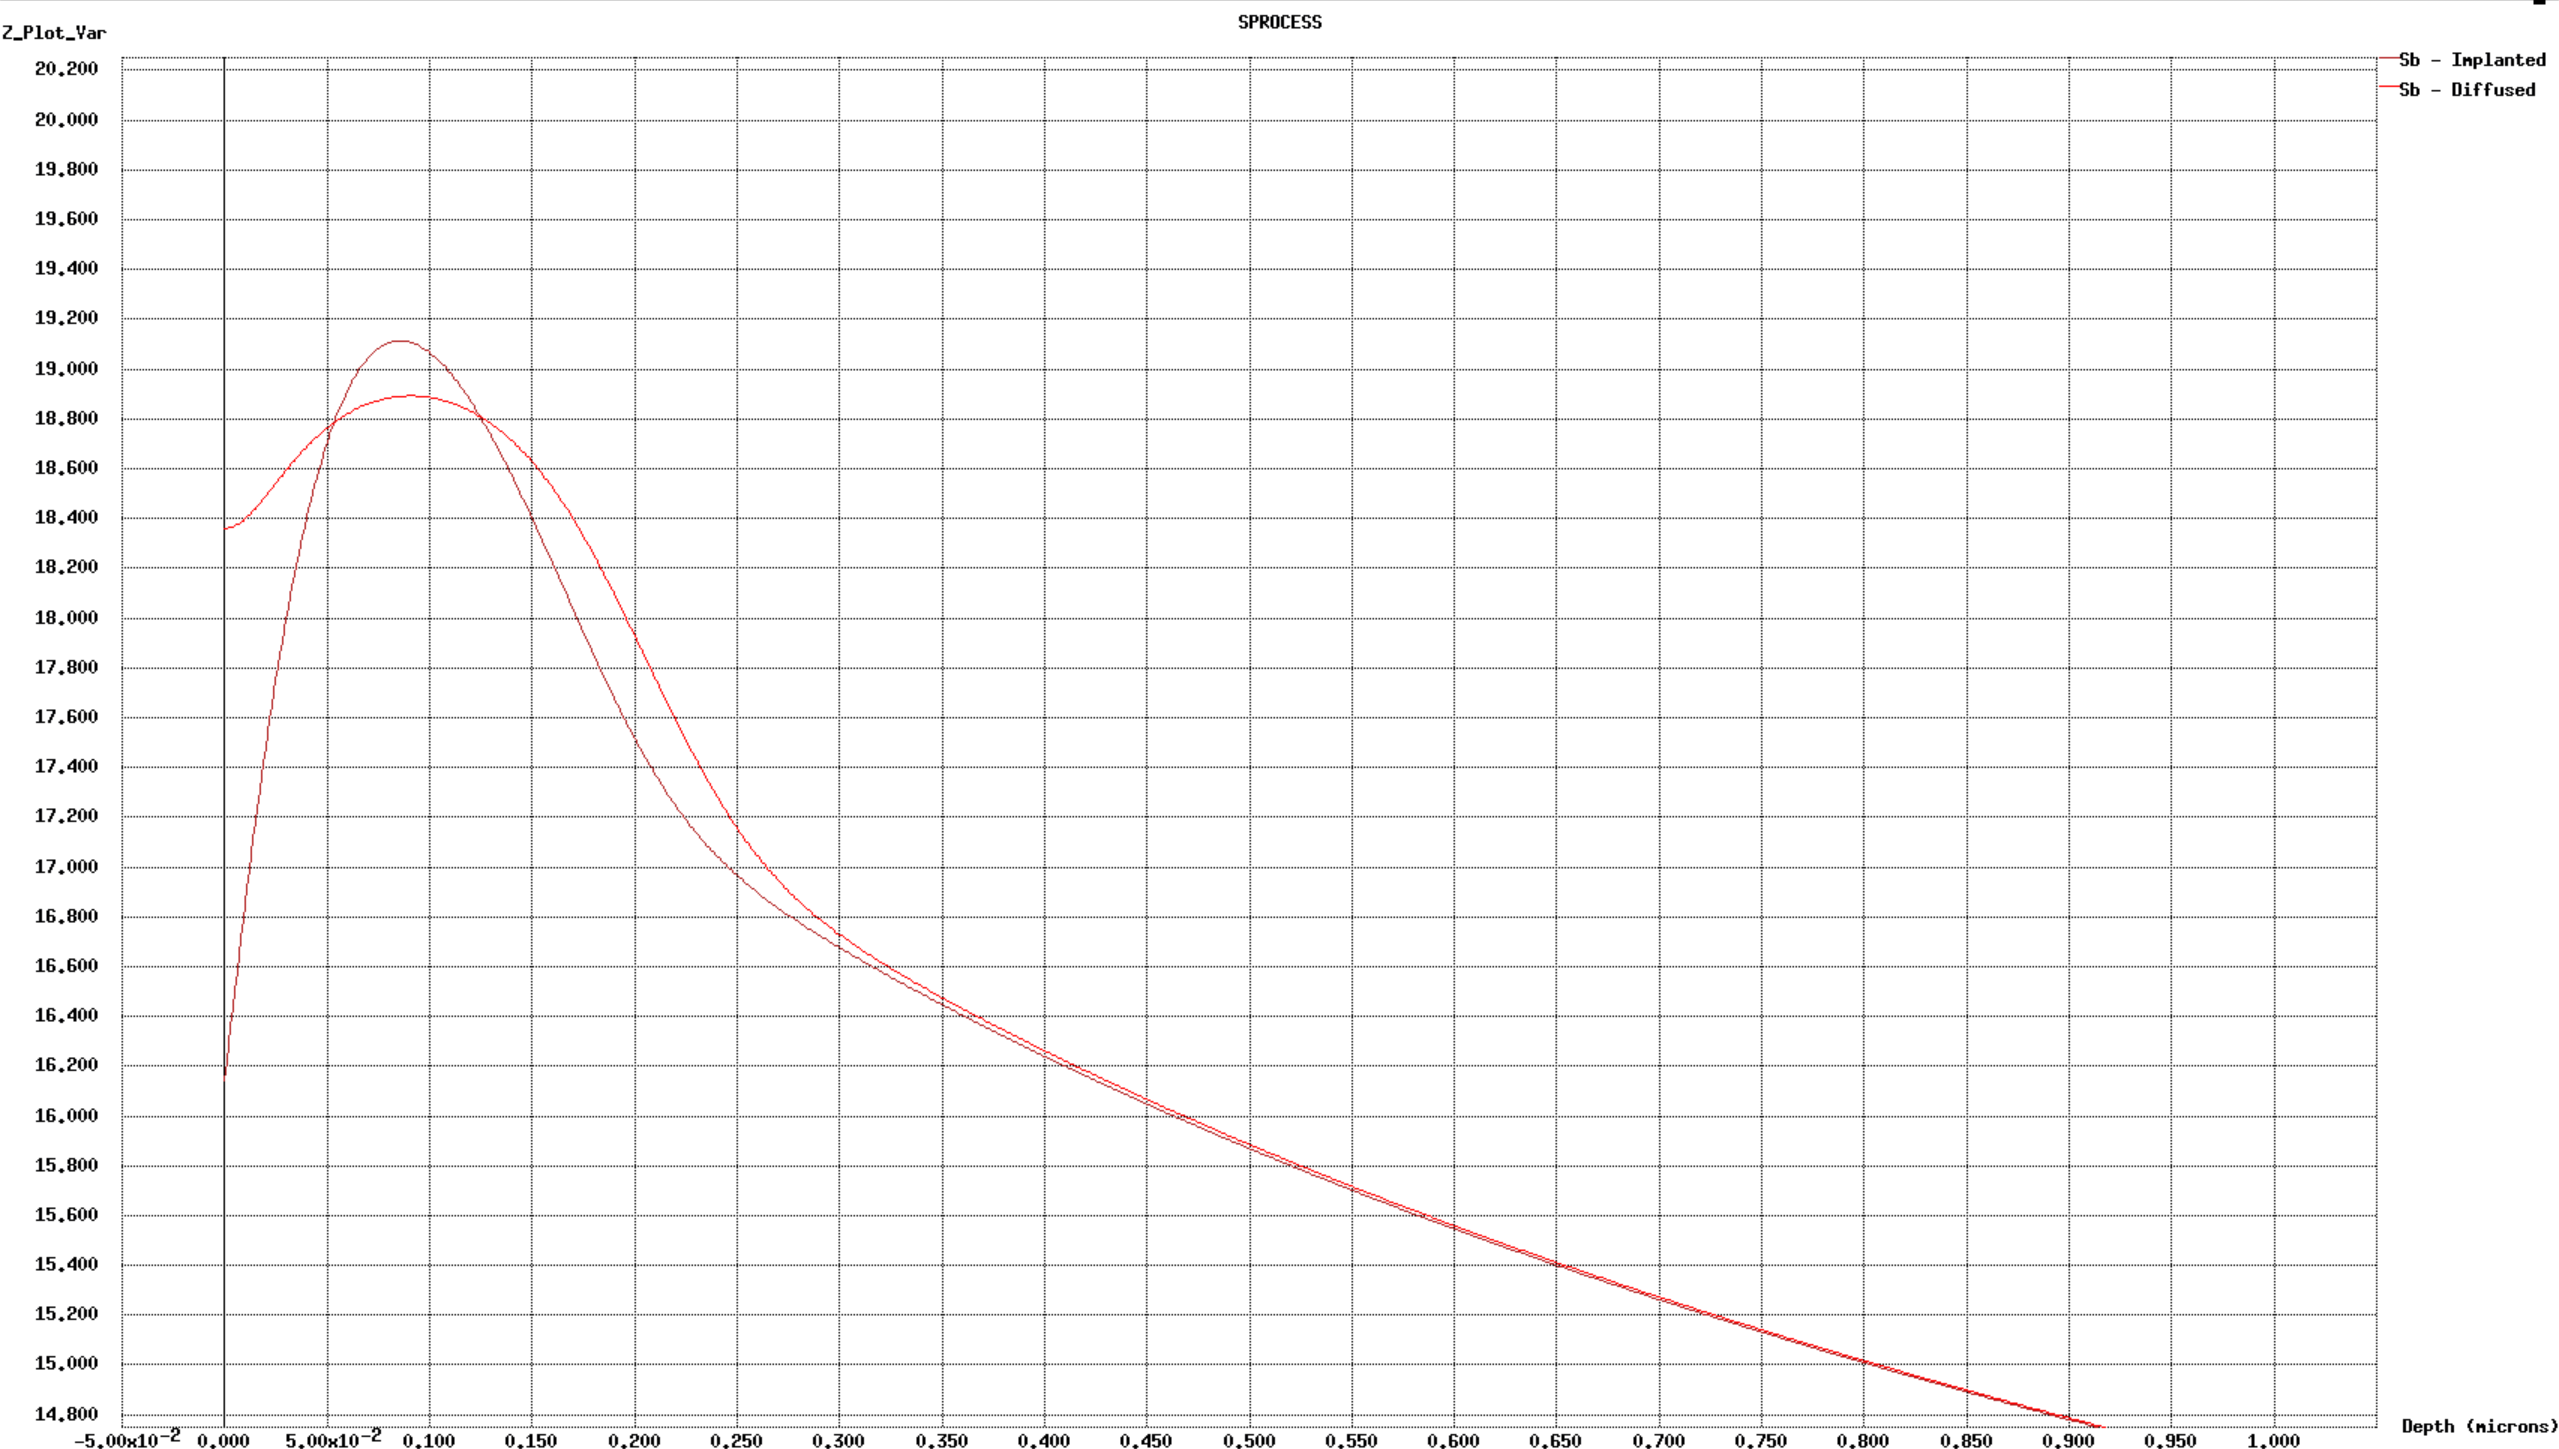
\includegraphics[width=0.75\linewidth]{Figures/impl_1e14.png}
    \caption{Antimony implantation and diffusion profile for a dose of
    $1\times10^{14}~\mathrm{cm^{-2}}$.}
    \label{fig:impl_1e14}
\end{figure}

\subsection{Process Simulation - 10}
\begin{table}[H]
    \centering
    \caption{Dopant ranking per property (1 = best, 4 = worst).}
    \label{tab:dopant-ranking}
    \begin{tabular}{lcccc}
        \toprule
        Dopant & Doping type & Short channeling tail & Narrow diffusion & Solid solubility \\
        \midrule
        Sb & n & 3 & 1 & 4 \\
        As & n & 4 & 2 & 1 \\
        P  & n & 2 & 4 & 2 \\
        B  & p & 1 & 3 & 3 \\
        \bottomrule
    \end{tabular}
\end{table}


 \subsection{Process Simulation - 11}
For the NMOS drain, a high dopant concentration and a sharp profile are required. Therefore, arsenic is the best choice. Arsenic is an n-type dopant with high solid
solubility, which allows a high active concentration. It also diffuses narrowly, which gives a highly doped and relatively sharp source/drain junction.

For the N-well, because the dopant must diffuse a few micrometers into the silicon with moderate concentration, phosphorus is the best choice. Phosphorus is an n-type dopant and diffuses deeper and wider than arsenic or antimony, making it suitable for forming a deep N-well. It also has a high solid solubility, so it can also meet the moderate concentration requirement easily.


\subsection{Process Simulation - 12}

\begin{figure}[H]
    \centering
    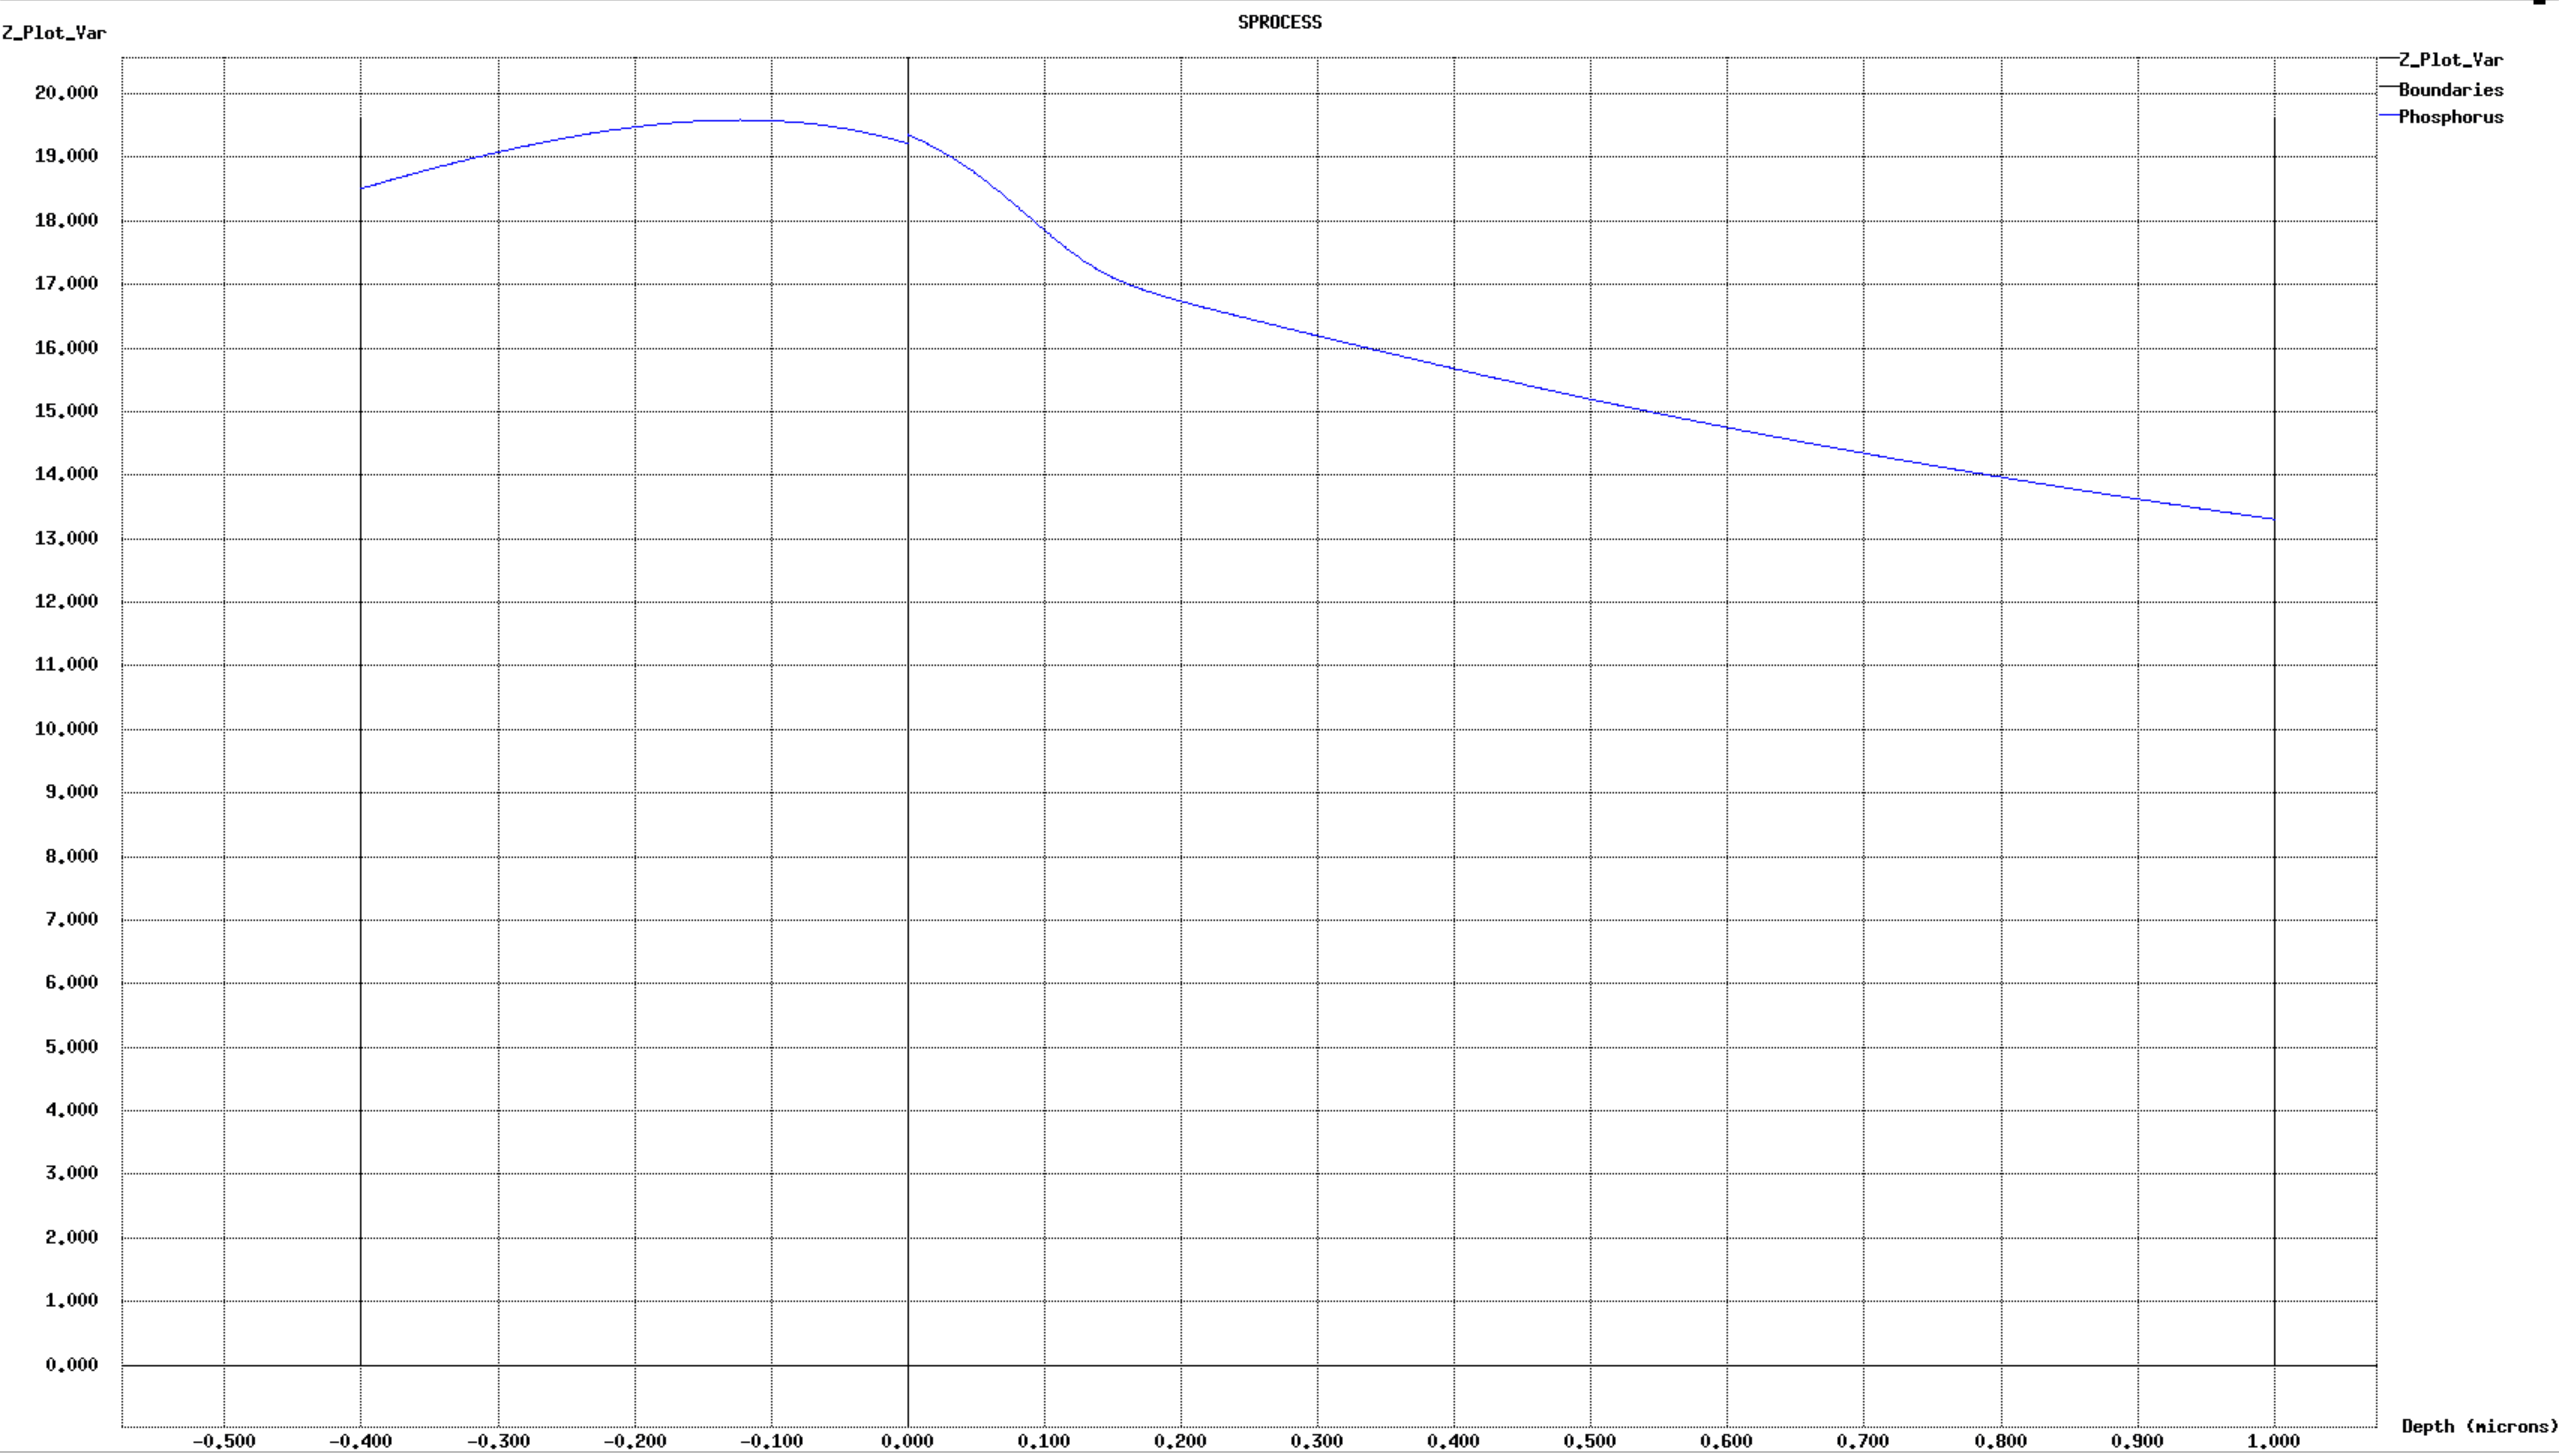
\includegraphics[width=0.7\linewidth]{Figures/resist_cmd.png}
    \caption{Phosphorus implantation profile through a $0.4~\mu\mathrm{m}$ photoresist mask.}
    \label{fig:resist_mask}
\end{figure}

The negative part of the x-axis of Fig. \ref{fig:resist_mask} represents the resist mask, because the phosphorus concentration is still present in the silicon region after passing through the resist. Therefore, a $0.4~\mu\mathrm{m}$ photoresist layer is not a sufficient implantation mask for this phosphorus implantation.

\subsection{Process Simulation - 13}

\begin{figure}[H]
    \centering
    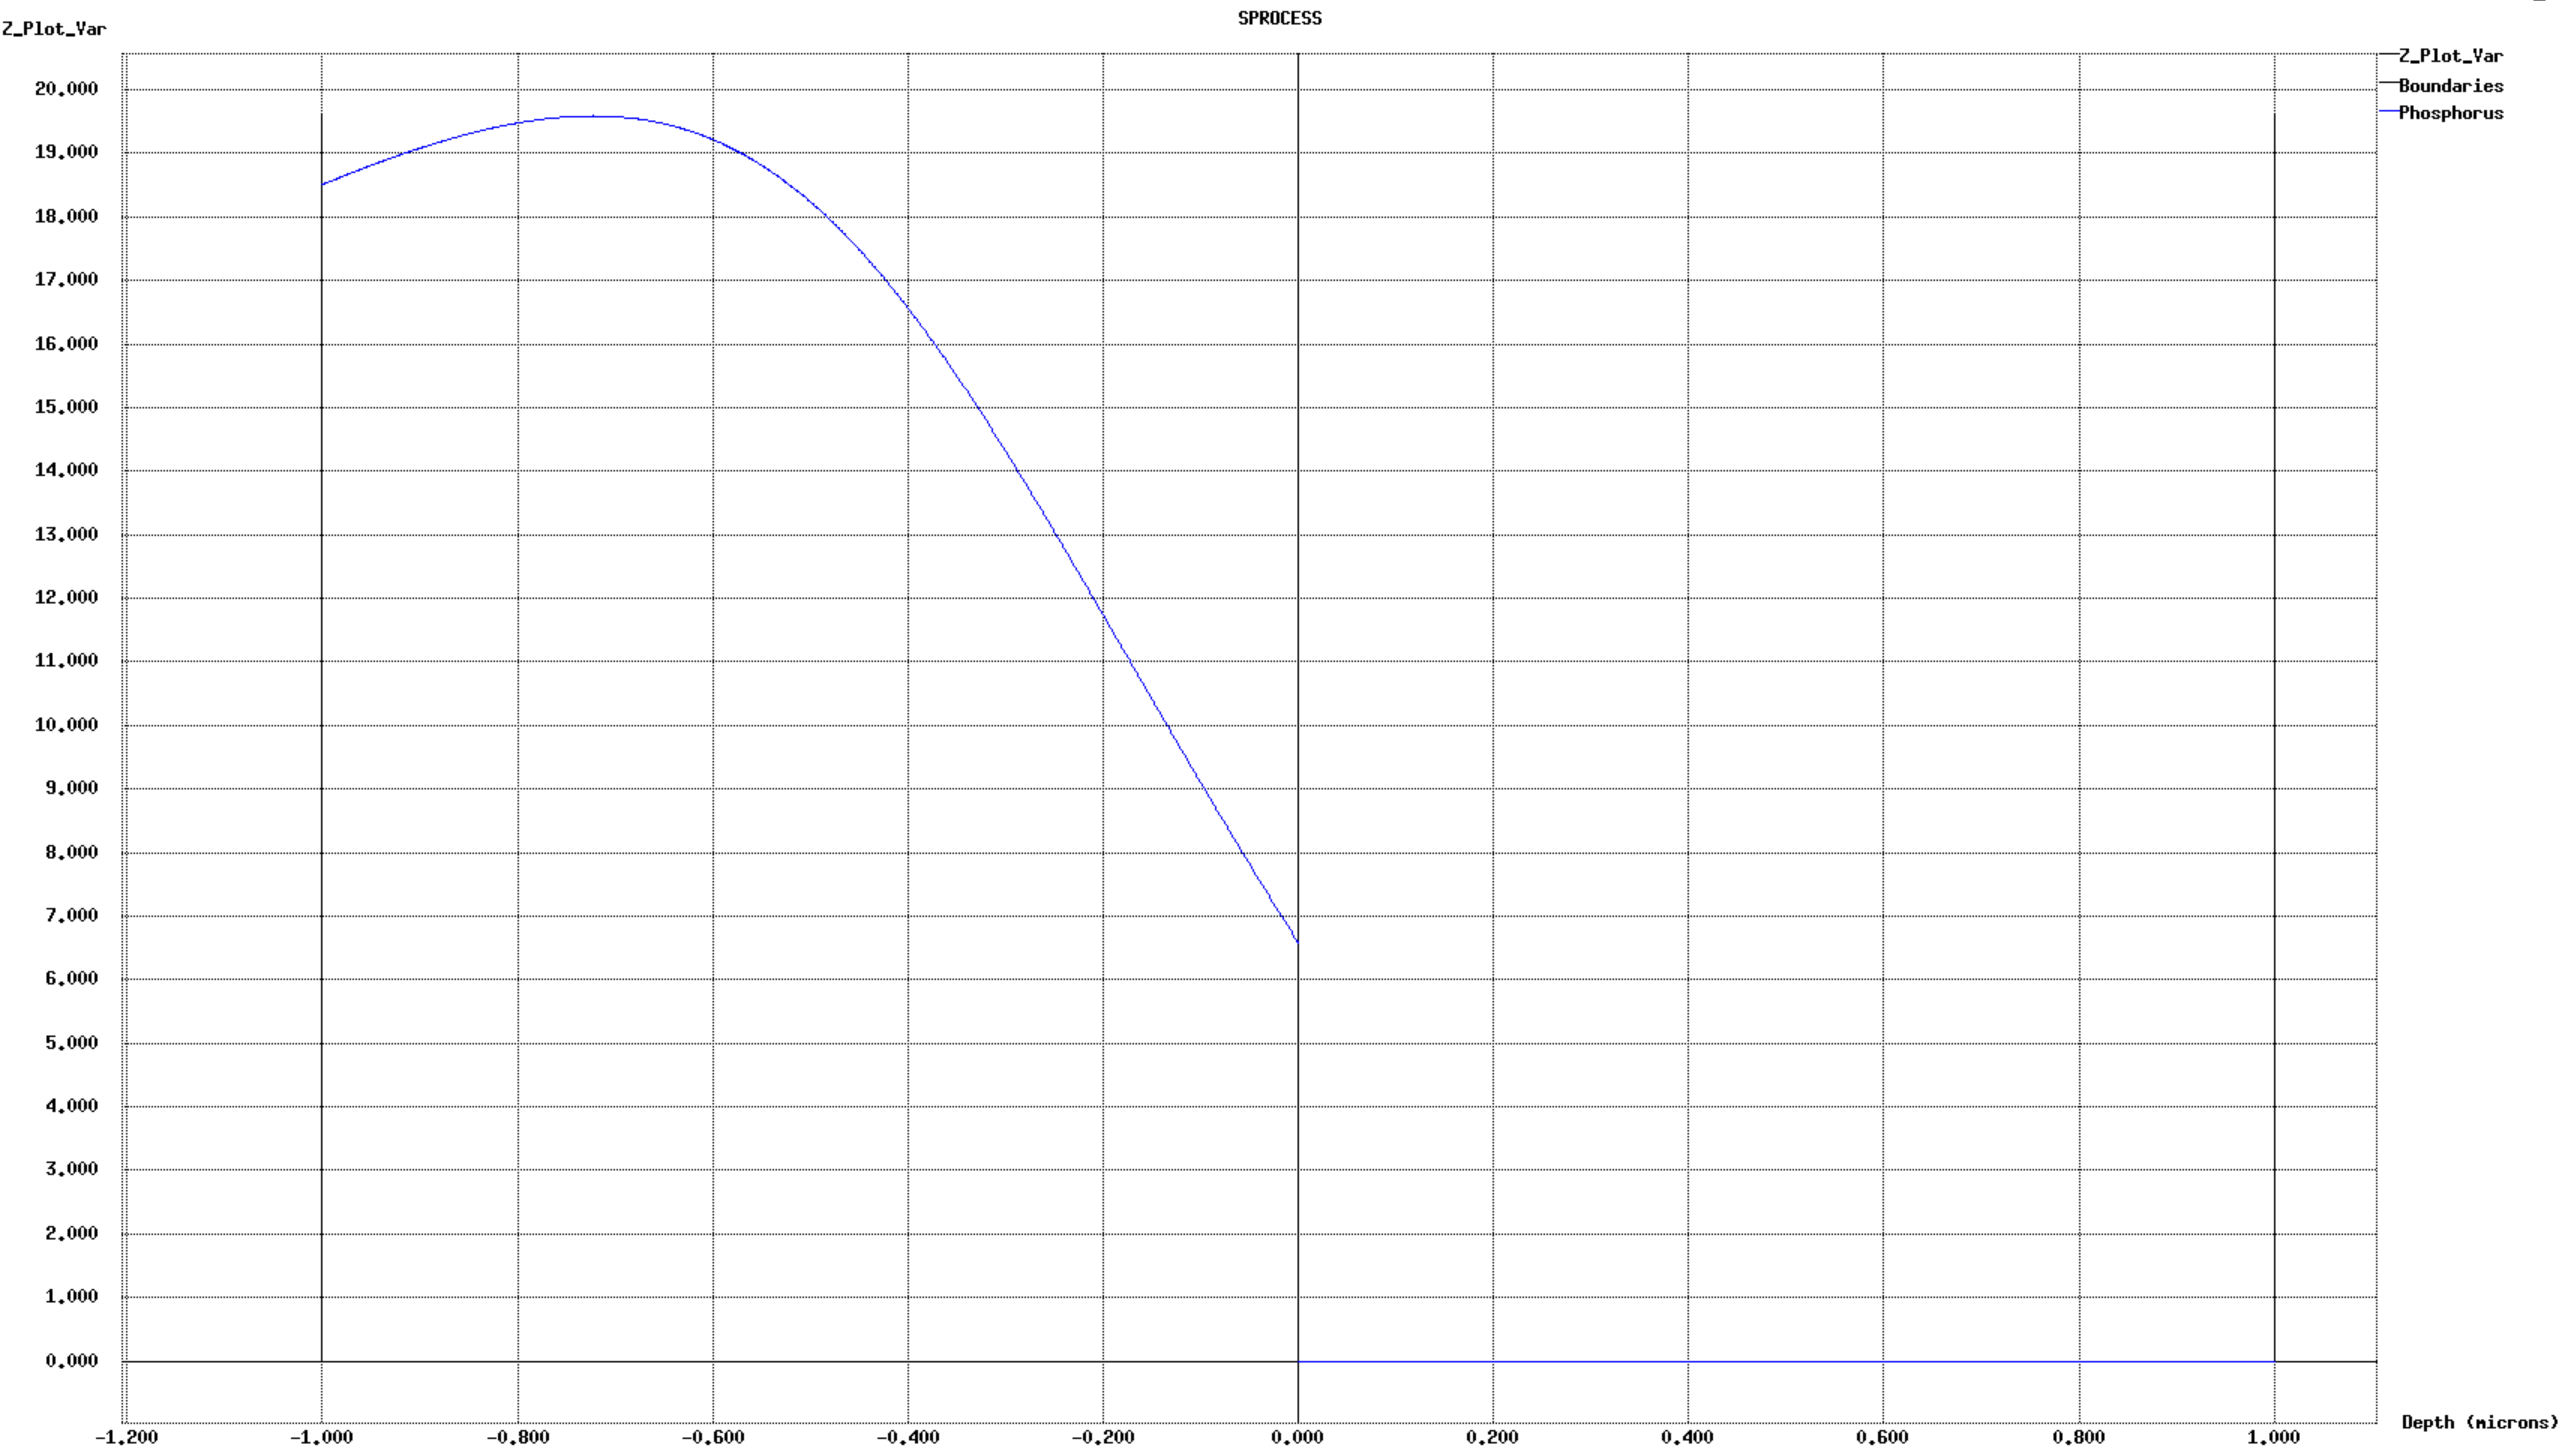
\includegraphics[width=0.7\linewidth]{Figures/resist_cmd_1000nm.png}
    \caption{Phosphorus implantation profile through a $1~\mu\mathrm{m}$ photoresist mask.}
    \label{fig:resist_mask_1000nm}
\end{figure}

After increasing the thickness of the photoresist layer from $0.4~\mu\mathrm{m}$ to $1~\mu\mathrm{m}$, the phosphorus concentration drops to zero before reaching the silicon region. Therefore, a $1~\mu\mathrm{m}$ photoresist layer is sufficient as an implantation mask for this phosphorus implantation.


\subsection{Process Simulation - 14 \& 15}

For the oxide mask, phosphorus ions still enter the silicon underneath. Therefore, an oxide layer with a thickness $0.4~\mu\mathrm{m}$ is insufficient.

\begin{figure}[H]
    \centering
    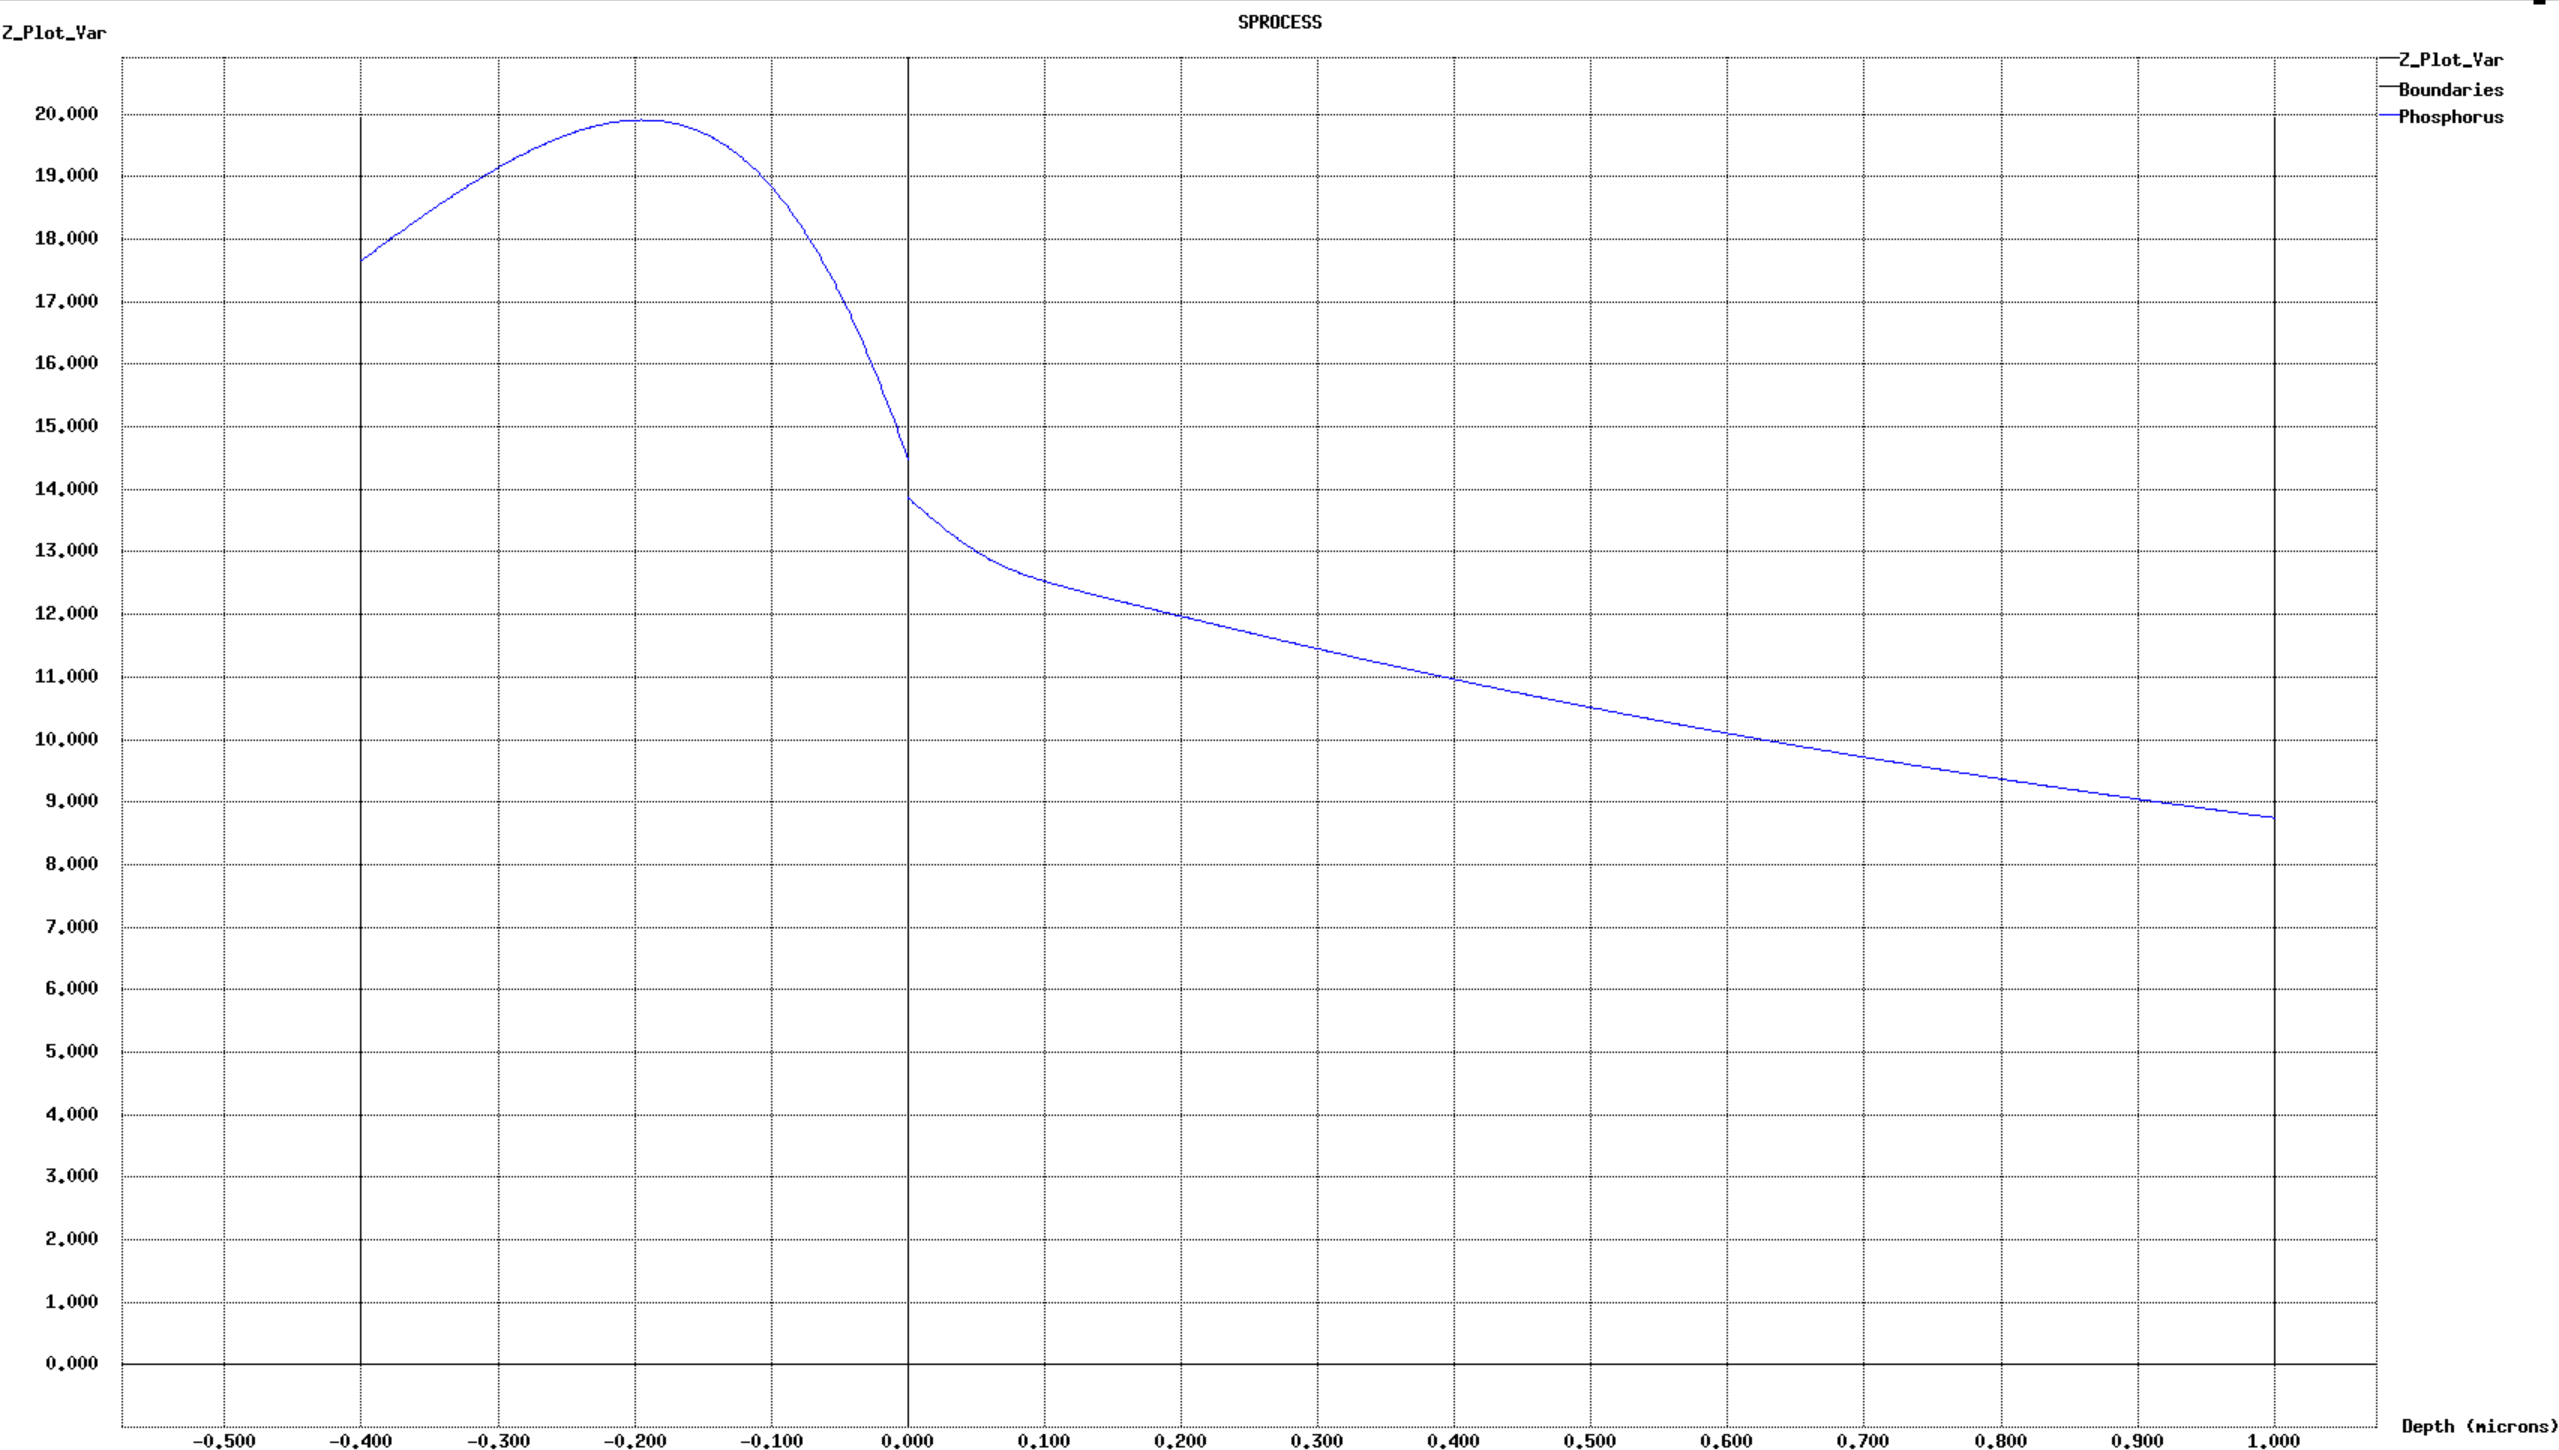
\includegraphics[width=0.7\linewidth]{Figures/oxide_cmd.png}
    \caption{Phosphorus implantation profile through an oxide mask.}
    \label{fig:oxide_mask}
\end{figure}

For the nitride mask, the Phosphorus concentration in the silicon is effectively zero. Therefore, in terms of stopping power, a $0.4~\mu\mathrm{m}$ thick nitride mask the most effective mask compared with oxide mask and photoresist mask with the same thickness.

\begin{figure}[H]
    \centering
    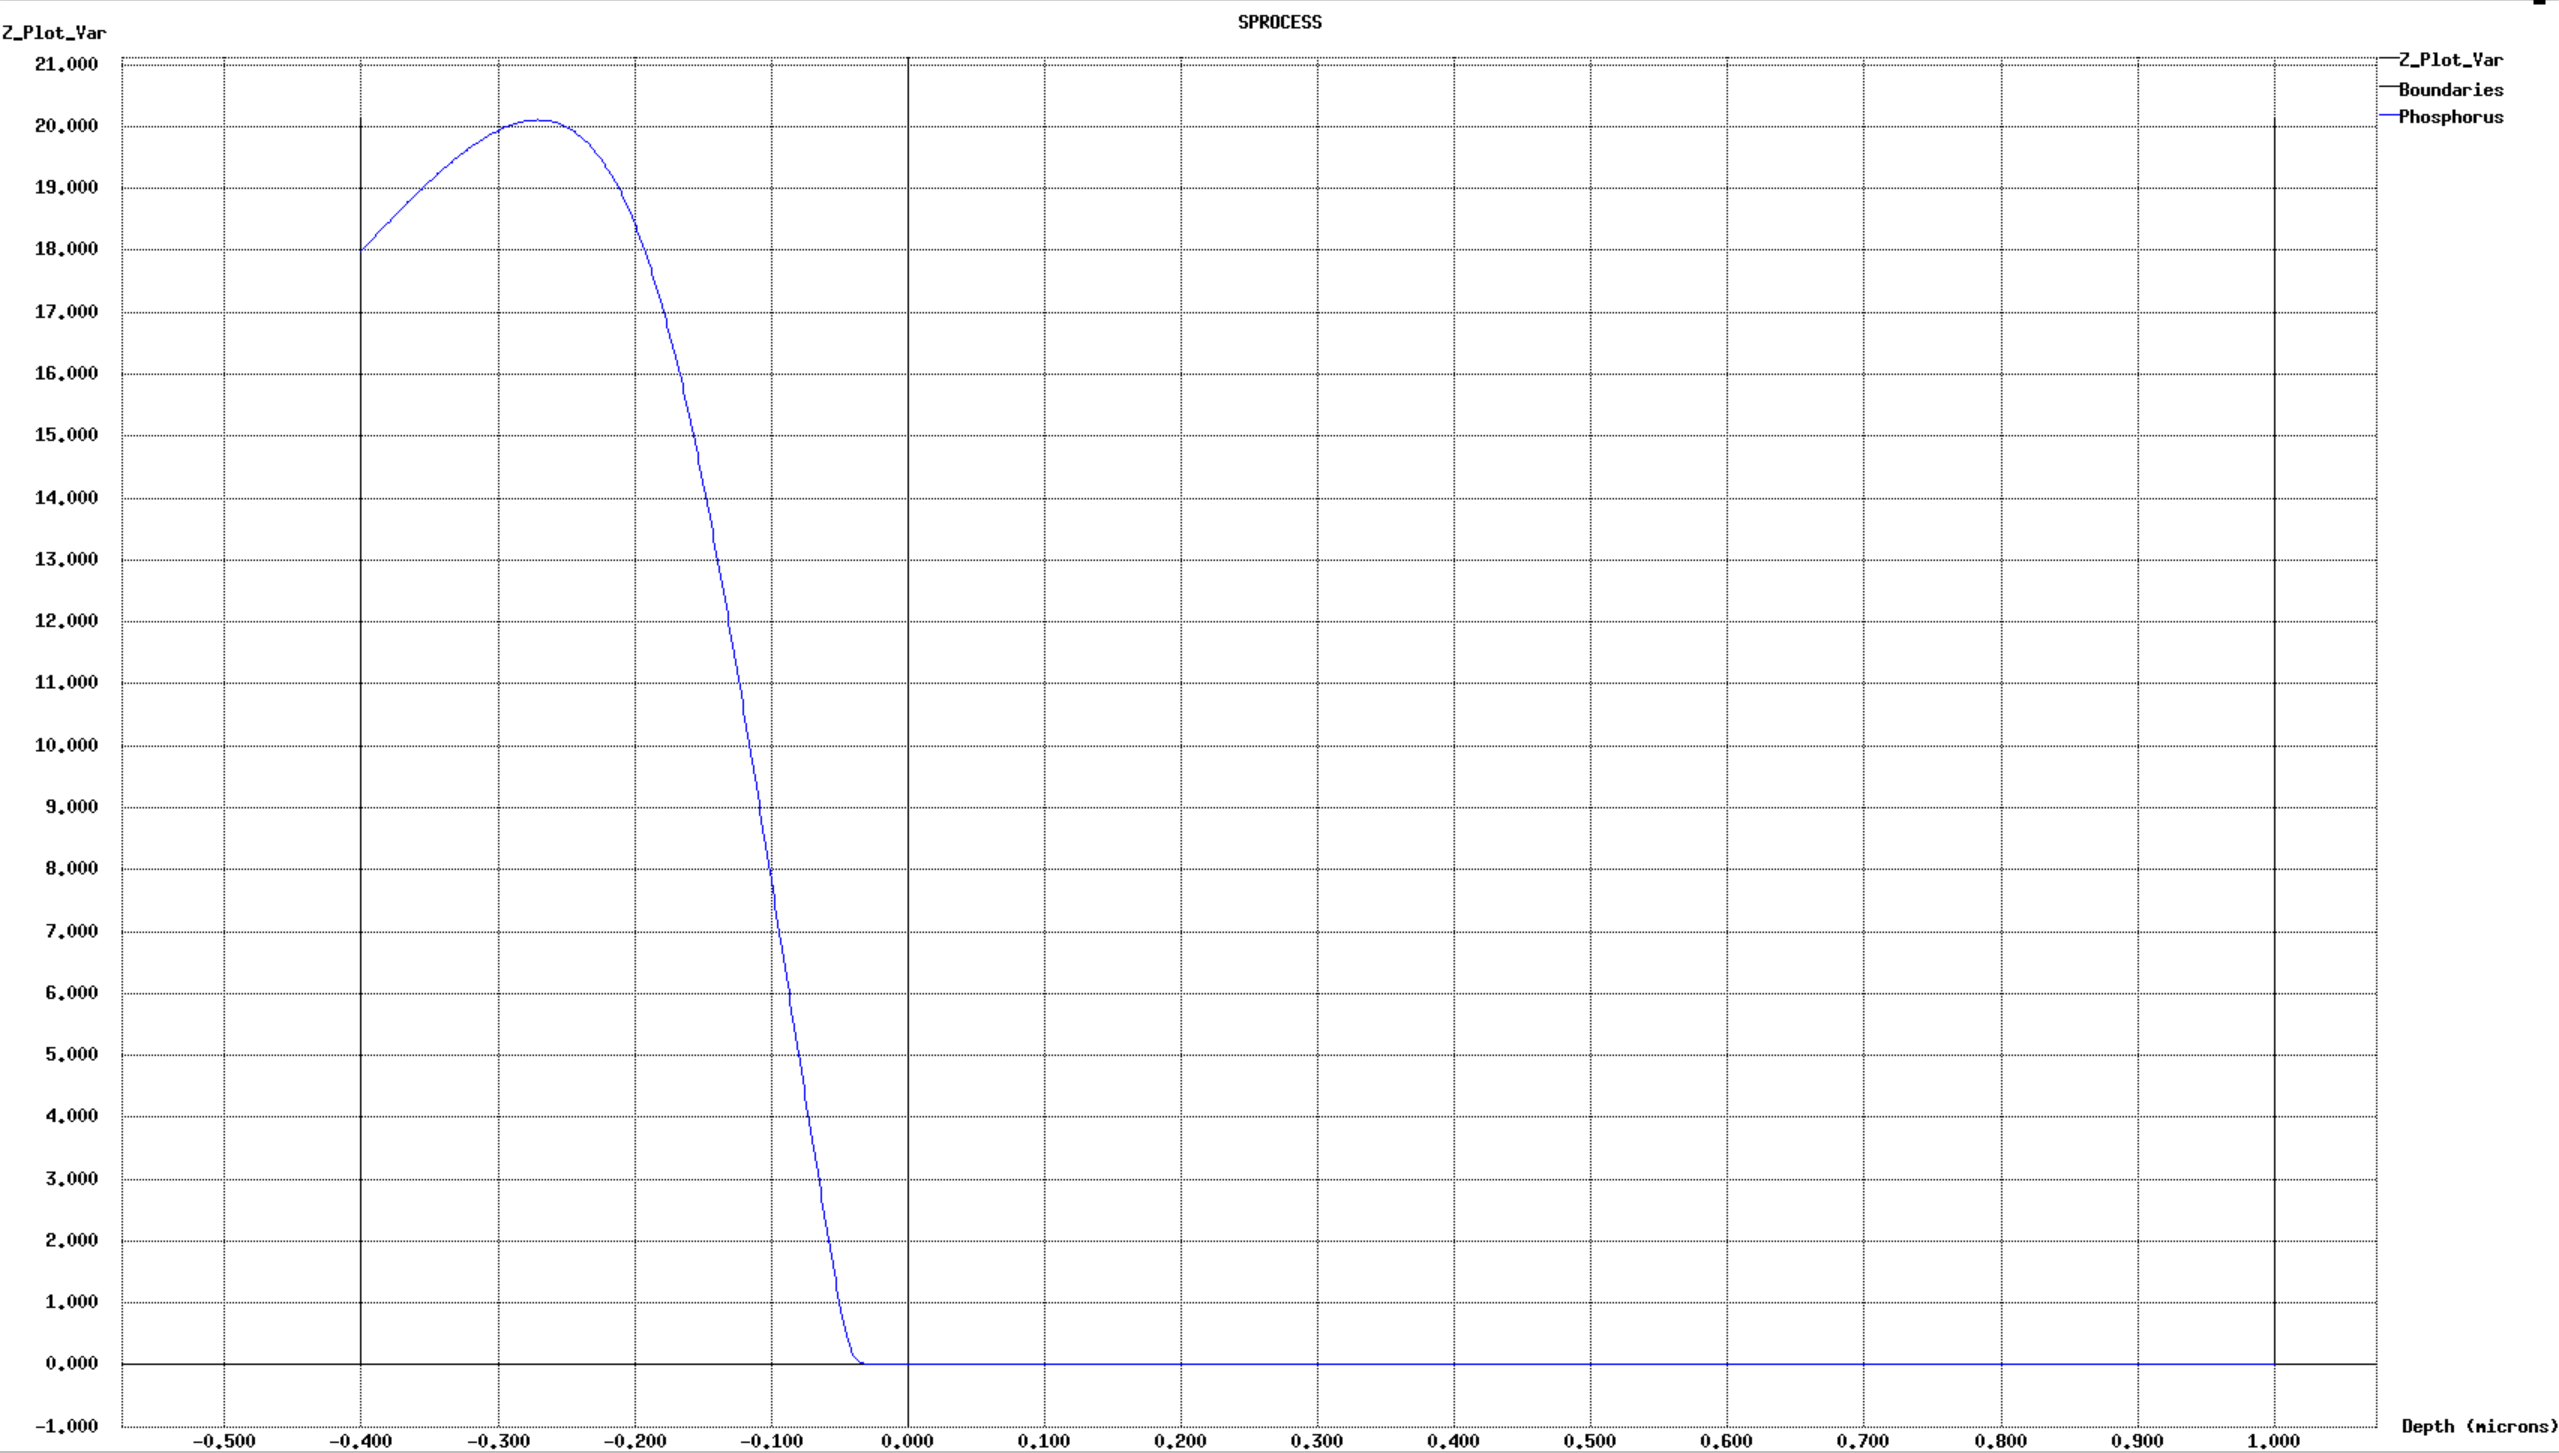
\includegraphics[width=0.7\linewidth]{Figures/nitride_cmd.png}
    \caption{Phosphorus implantation profile through a nitride mask.}
    \label{fig:nitride_mask}
\end{figure}

Nitride is almost never used as a standard implantation mask because a nitride layer is deposited at high temperatures, which means it is hard to process. In addition, it is difficult to pattern and remove. Because of its high intrinsic tensile stress, it can also introduce stress in the wafer.

In standard processing, photoresist is used most often because it is easy to pattern. Although photoresist has relatively low stopping power, it can be made thick enough to absorb the ions so that none reach the silicon. Finally, it can be removed easily after implantation.

\section{Device simulation}
\subsection{Device Simulation - 4}
For NMOS, the 2D cross-section of the NMOS generated by SVisual generally matches the reference cross-section from the manual. In the reference cross-section, the source, drain, substrate contact, oxide, and metal regions are drawn as ideal rectangular shapes. While the visualization result depicts a more realistic view. The doped regions are not rectangular and the doping concentration also changes gradually with depth instead of having a defined boundary.

\begin{figure}[H]
    \centering
    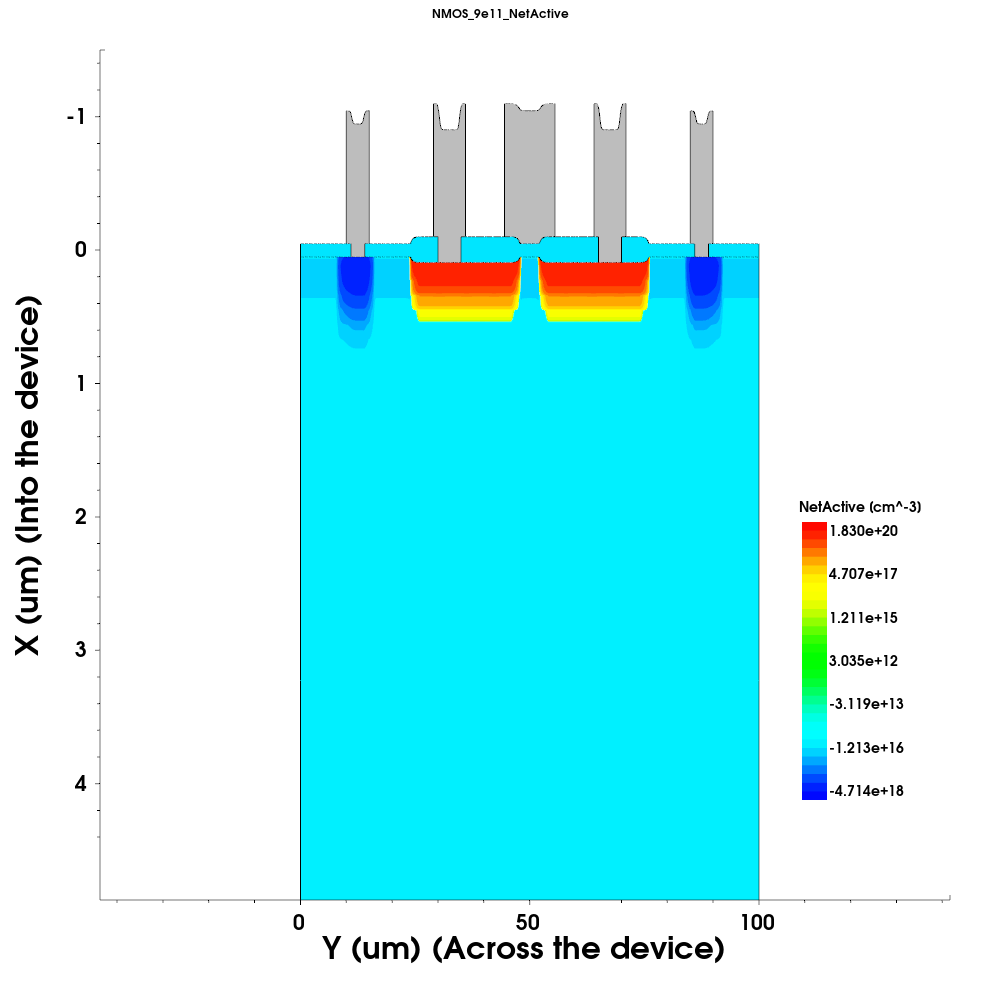
\includegraphics[width=0.4\textwidth]{Figures/NMOS_9e11_deviceStructure.png}
    \caption{Simulated NMOS cross-section showing the net active dopant concentration for a VT-adjust dose of $9\times10^{11}~\mathrm{cm^{-2}}$.}
    \label{fig:nmos_cross_section}
\end{figure}

For PMOS, the 2D cross-section of the PMOS generated by SVisual also generally matches the reference cross-section from the manual.
\begin{figure}[H]
    \centering
    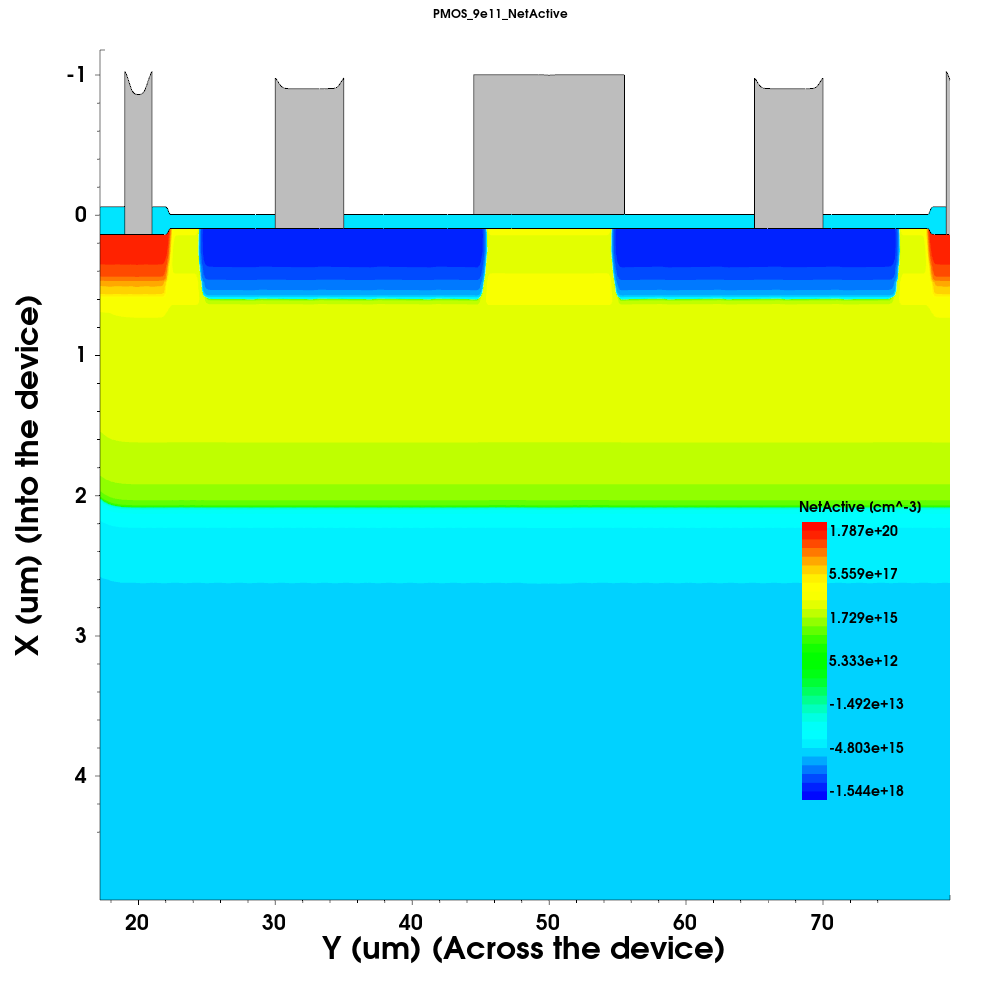
\includegraphics[width=0.4\textwidth]{Figures/PMOS_9e11_deviceStructure.png}
    \caption{Simulated PMOS cross-section showing the net active dopant concentration for a VT-adjust dose of $9\times10^{11}~\mathrm{cm^{-2}}$.}
    \label{fig:pmos_cross_section}
\end{figure}

\subsection{Device Simulation - 5}
The simulated profiles are net active doping profiles. In the NMOS, the source and drain are n-type SN regions, while the channel and substrate are p-type. In the PMOS, the device is located inside the n-type N-well, and the source and drain are p-type SP regions.

The simulated junction depths were extracted from the .csv files generated by finding where the signed net active doping crosses zero. The extracted values are $0.537~\mu\mathrm{m}$ for SN, $2.085~\mu\mathrm{m}$ for the N-well, and $0.594~\mu\mathrm{m}$ for SP.

The simulated values differ from the calculated values because the calculations in Chapter 2 assume the implantation profiles follow Gaussian distribution and there is no subsequent thermal steps, while the simulation includes the full process flow and dopant redistribution during the thermal steps.

Simulation results shows that the depth of SN and SP are much deeper than calculated.

Meanwhile, N-WELL is simulated slightly shallower than calculated.


\begin{table}[H]
    \centering
    \caption{Junction depth: analytical (Chapter 2) vs Sentaurus simulation.}
    \label{tab:xj}
    \begin{tabular}{lcc}
        \toprule
        Implantation & Calc. junction depth ($\mu$m) & Simulated junction depth ($\mu$m) \\
        \midrule
        SN     & 0.087 & 0.54 \\
        N-WELL & 2.37  & 2.09 \\
        SP     & 0.186 & 0.59 \\
        \bottomrule
    \end{tabular}
\end{table}


\subsection{Device Simulation - 6}
\begin{figure}[h]
    \centering
    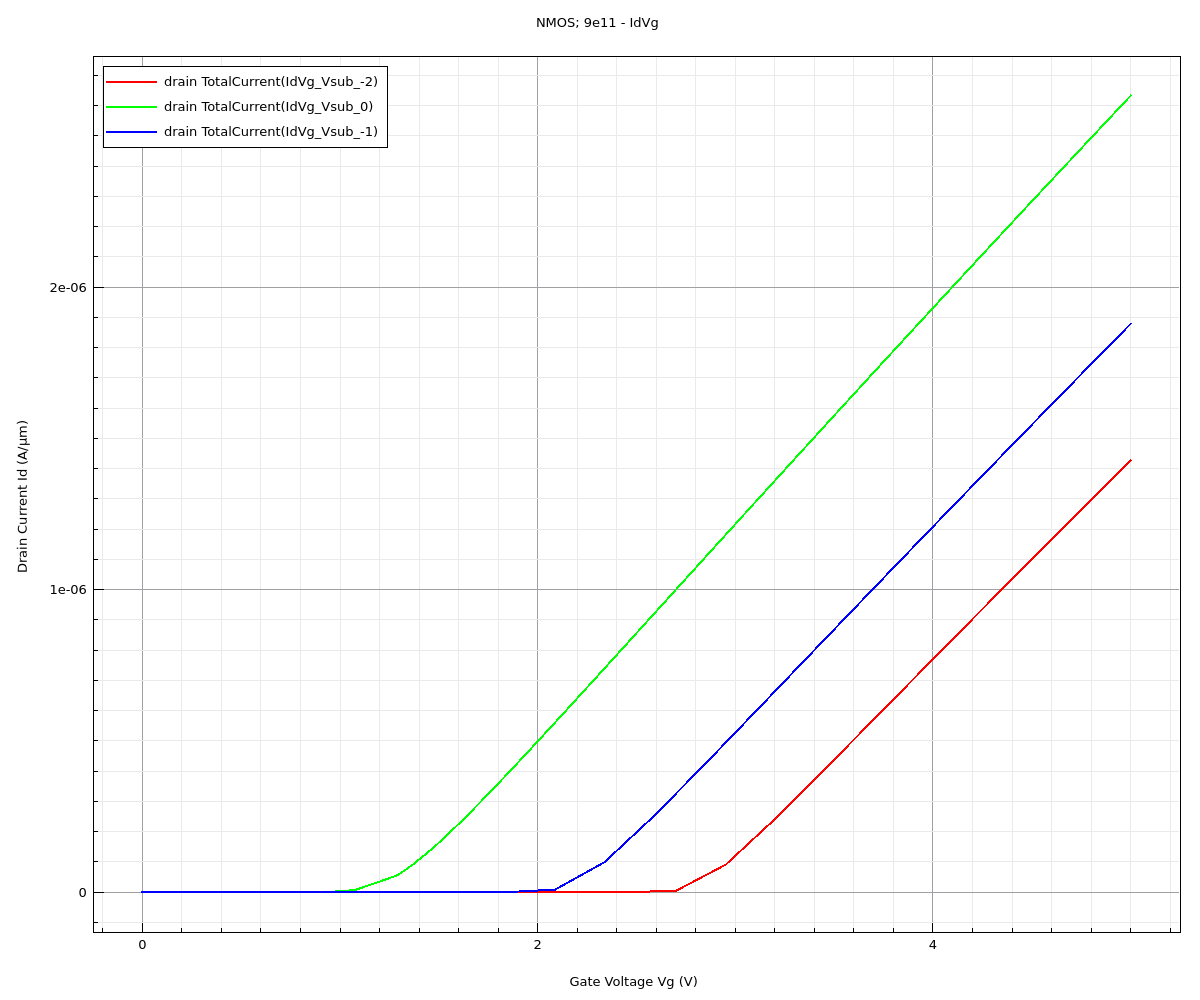
\includegraphics[width=0.8\linewidth]{Figures/NMOS_9e11_IdVg.png}
    \caption{Simulated NMOS $I_D$--$V_G$ characteristics at $V_D = 0.1$~V for substrate bias $V_\text{Sub} = 0$, $-1$, and $-2$~V ($V_T$-adjust dose $9 \times 10^{11}$~cm$^{-2}$).}
    \label{fig:nmos-idvg}
\end{figure}

The threshold voltage is extracted from the exported $I_D$--$V_G$ data by linear extrapolation at maximum transconductance. In the linear region (small $V_D$) the drain current is
\begin{gather*}
I_D = \mu_n C_\text{ox} \frac{W}{L}\left(V_{GS} - V_T - \frac{V_{DS}}{2}\right) V_{DS},
\end{gather*}
which is linear in $V_{GS}$. Extrapolating the tangent taken at the point of maximum
transconductance $(V_{GS}^{\prime}, I_D^{\prime})$ to $I_D = 0$ gives the intercept
$V_{GS0} = V_T + V_{DS}/2$, so
\begin{gather*}
V_T = V_{GS0} - \frac{V_DS}{2}, \qquad \frac{V_{DS}}{2} = 0.05~\text{V}.
\end{gather*}
where the intercept is evaluated from the data as
\begin{gather*}
V_{GS0} = V_{GS}^{\prime} - \frac{I_D^{\prime}}{g_{m,\text{max}}},
\qquad
g_{m,\text{max}} = \max\!\left(\frac{\Delta I_D}{\Delta V_{GS}}\right).
\end{gather*}

This yields $V_T = 1.26$, $2.17$, and $2.78$~V for $V_\text{Sub} = 0$, $-1$, and $-2$~V, respectively.

The threshold voltage increases as $V_\text{Sub}$ becomes more negative. This is the body effect: a more negative $V_\text{Sub}$ raises the reverse source-body bias $V_{SB} = -V_\text{Sub}$, widening the channel-substrate depletion region and adding depletion charge that the gate must balance before inversion. This matches the theory of the body effect,
\begin{gather*}
V_T = V_{T0} + \gamma\left(\sqrt{2\phi_F + V_{SB}} - \sqrt{2\phi_F}\right),
\end{gather*}
where $V_T$ rises with $V_{SB}$, consistent with the simulated trend.

\begin{figure}[H]
    \centering
    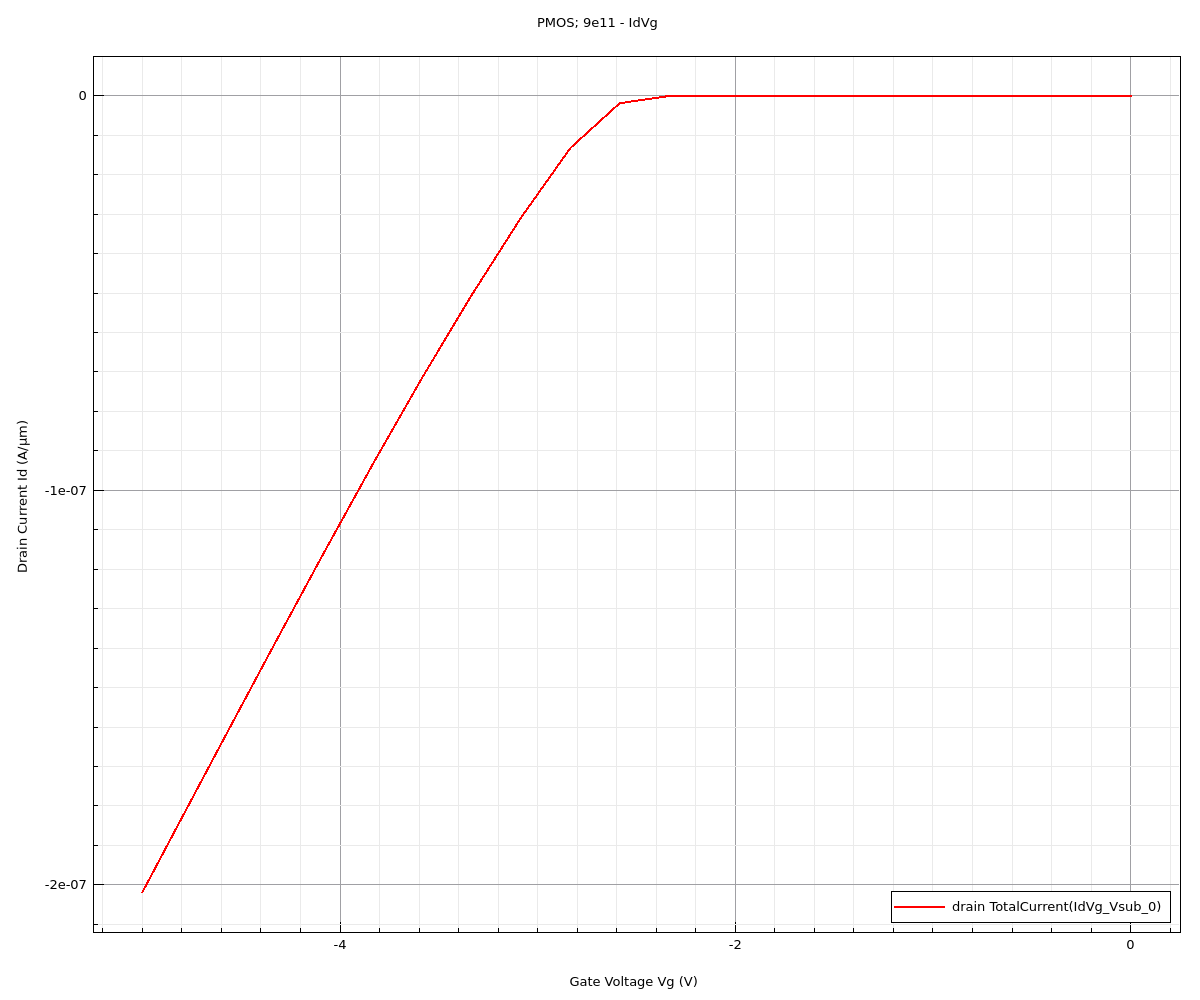
\includegraphics[width=0.8\linewidth]{Figures/PMOS_9e11_IdVg.png}
    \caption{Simulated PMOS $I_D$--$V_G$ characteristics at $V_D = -0.1$~V for substrate bias $V_\text{Sub} = 0$~V ($V_T$-adjust dose $9 \times 10^{11}$~cm$^{-2}$).}
    \label{fig:pmos-idvg}
\end{figure}

The PMOS is simulated only at $V_\text{Sub} = 0$~V. Applying the same method with $V_D/2 = -0.05$~V gives a threshold voltage of $V_T = -2.81$~V.





\subsection{Device Simulation - 7}
Figure~\ref{fig:nmos-idvd} shows one curve per gate voltage, so $V_G$ is the parameter that changes from line to line. The curves for $V_G \le 1$~V stay near zero because the device is below threshold ($V_T \approx 1.26$~V). Each conducting curve first rises almost proportionally to $V_{DS}$ (linear region), then flattens once $V_{DS}$ passes the knee at $V_{DS} \approx V_G - V_T$ (saturation region). The knee shifts to higher $V_{DS}$ as $V_G$ increases. For $V_G = 6$ and $7$~V it falls beyond the swept range, so those curves are still rising at $V_{DS} = 5$~V and do not fully saturate.

The saturation current follows the long-channel square law $I_{D,\text{sat}} \propto (V_G - V_T)^2$. The ratio $I_D/(V_G - V_T)^2$ at $V_{DS} = 5$~V stays close to $2.6 \times 10^{-6}$ over $V_G = 3$ to $7$~V, and the gap between successive curves widens with $V_G$. Velocity saturation would instead make the current linear in $V_G - V_T$, giving roughly equal spacing. That is not seen here. The saturated curves are nearly flat, so channel-length modulation is small. The device
therefore shows no velocity saturation or other short-channel effects, as expected for its long channel.

\begin{figure}[H]
    \centering
    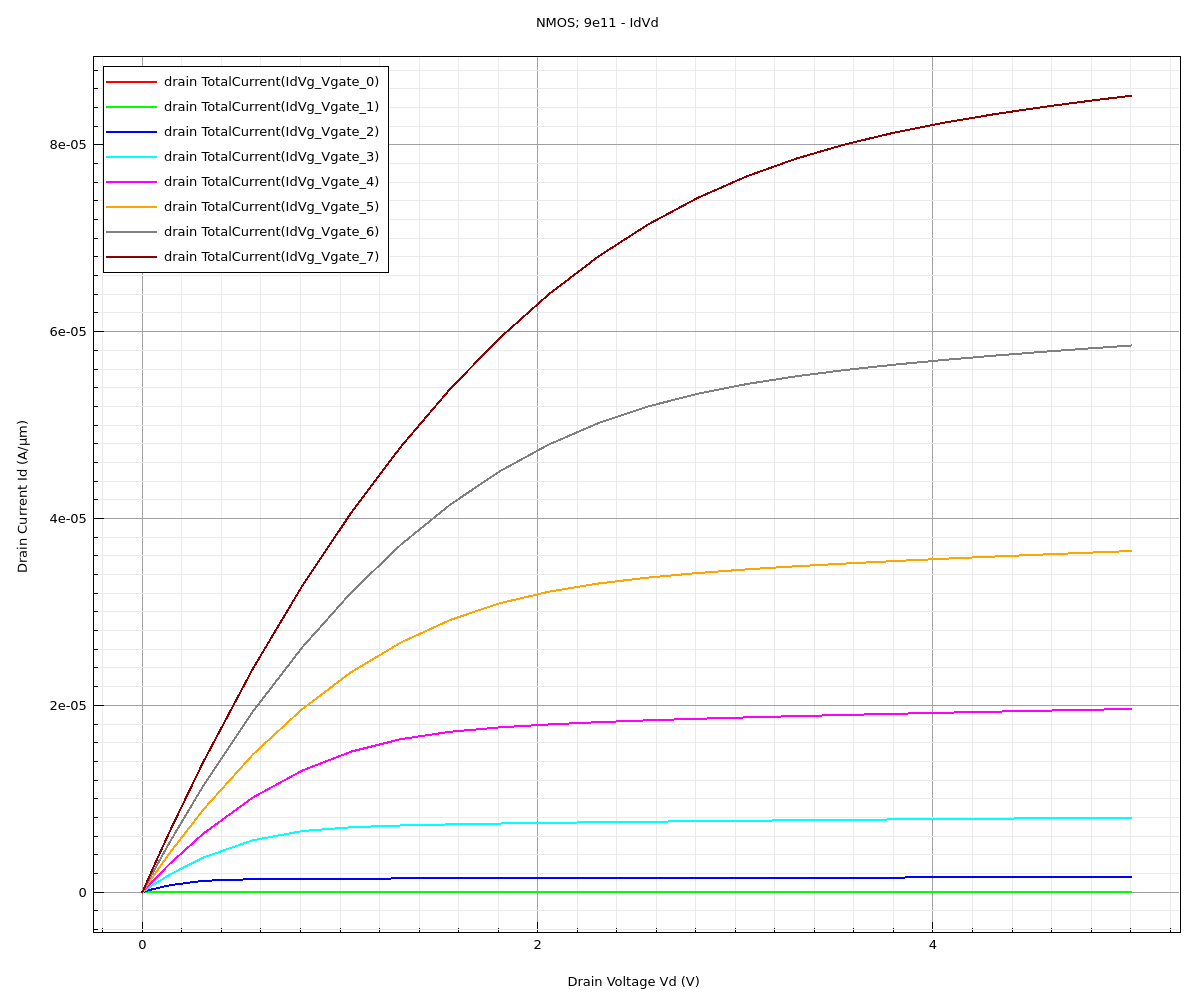
\includegraphics[width=0.8\linewidth]{Figures/NMOS_9e11_IdVd.png}
    \caption{Simulated NMOS $I_D$--$V_{DS}$ characteristics for $V_G = 0$ to $7$~V in
    $1$~V steps at $V_\text{Sub} = 0$ ($V_T$-adjust dose $9 \times 10^{11}$~cm$^{-2}$).}
    \label{fig:nmos-idvd}
\end{figure}


The PMOS characteristics in Figure~\ref{fig:pmos-idvd} show the same behaviour. The linear and saturation regions and the square-law spacing match the NMOS case, and the curves show no short-channel effects. At equal $|V_G|$ the PMOS currents are smaller in magnitude than the NMOS currents, because the hole mobility is lower than the electron mobility and the larger PMOS threshold magnitude ($V_T \approx -2.81$~V) leaves less gate overdrive.

\begin{figure}[H]
    \centering
    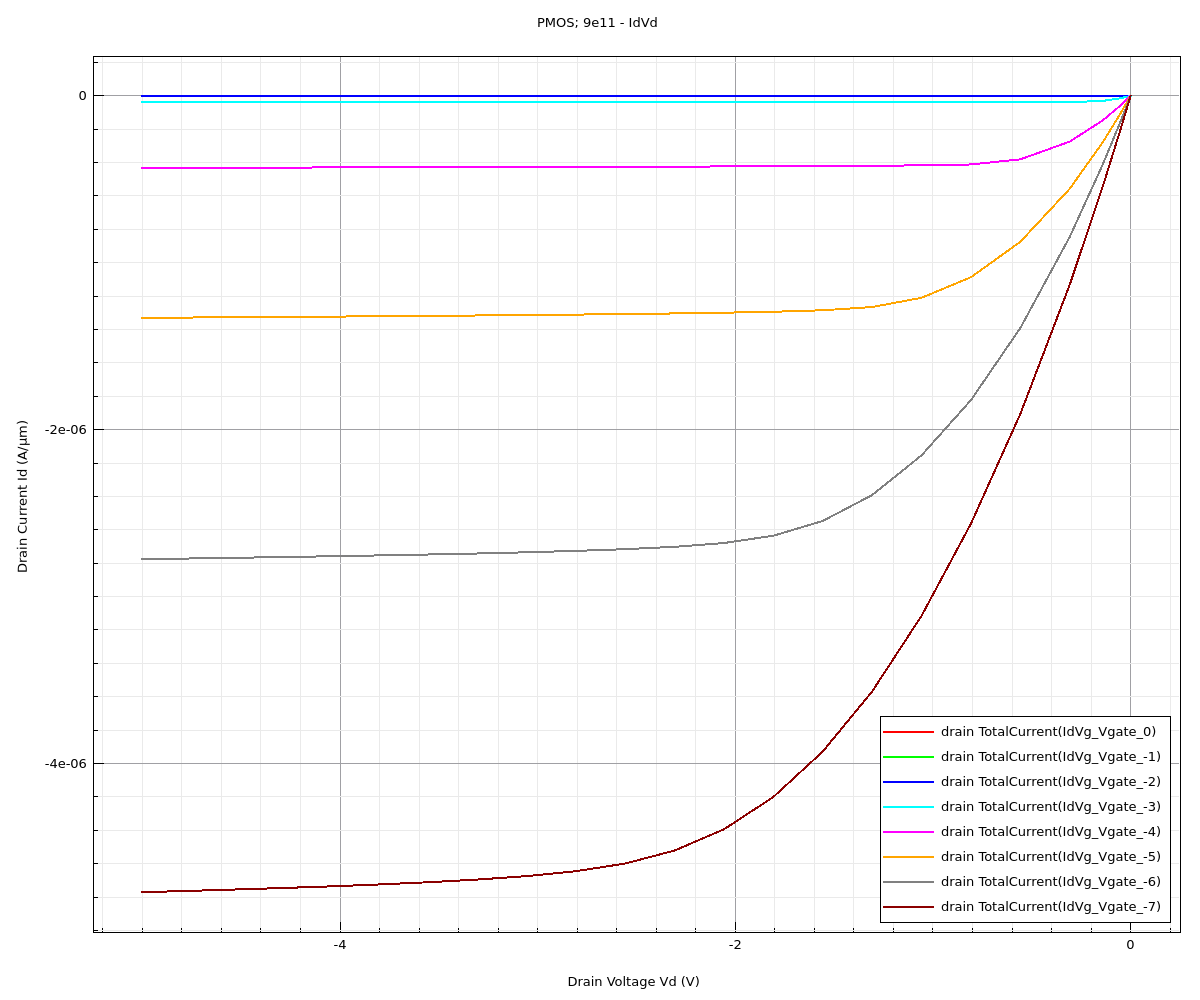
\includegraphics[width=0.8\linewidth]{Figures/PMOS_9e11_IdVd.png}
    \caption{Simulated PMOS $I_D$--$V_{DS}$ characteristics for $V_G = 0$ to $-7$~V in
    $1$~V steps at $V_\text{Sub} = 0$ ($V_T$-adjust dose $9 \times 10^{11}$~cm$^{-2}$).}
    \label{fig:pmos-idvd}
\end{figure}


\subsection{Device Simulation - 9}
\begin{figure}[H]
    \centering
    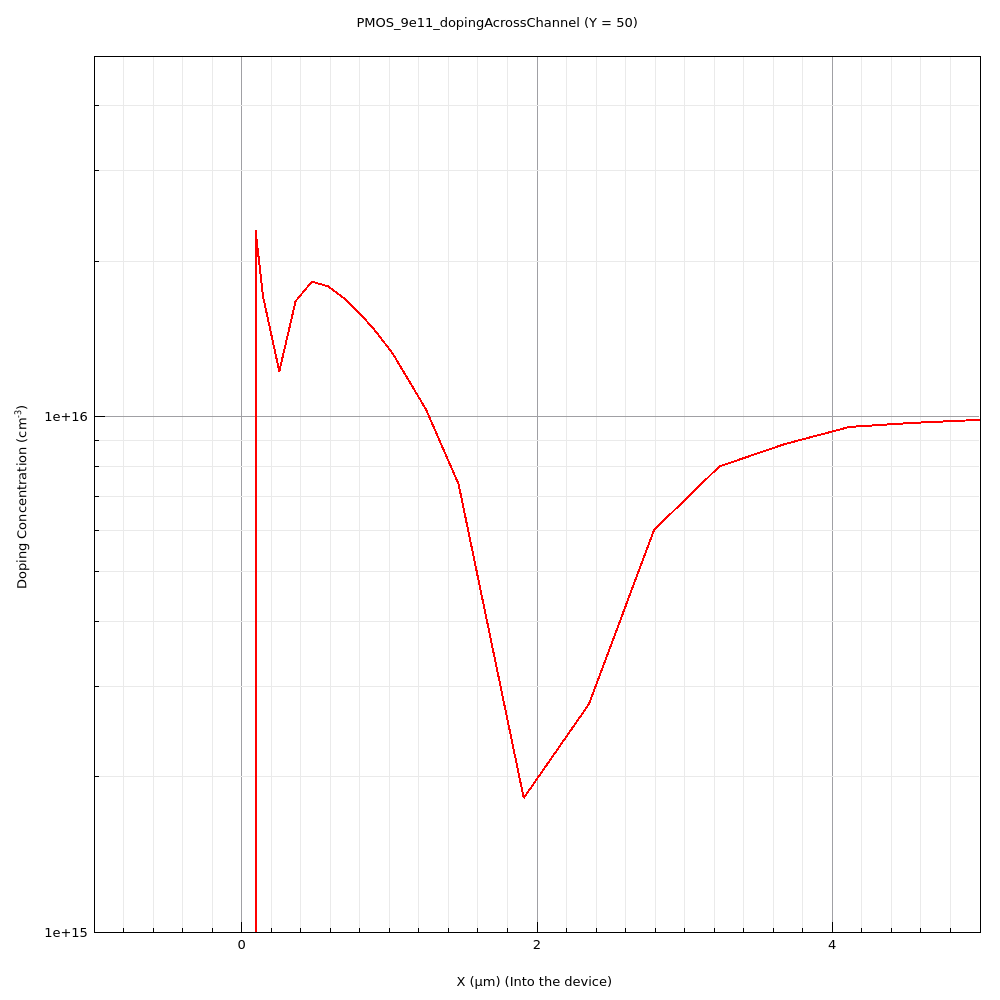
\includegraphics[width=0.5\textwidth]{Figures/PMOS_9e11_dopingAcrossChannel.png}
    \caption{Simulated PMOS dopant concentration across the channel for a VT-adjust dose of $9\times10^{11}~\mathrm{cm^{-2}}$.}
    \label{fig:pmos_cross_section}
\end{figure}

For the PMOS, after changing the the dose from 9e11 at/$\text{cm}^2$ to 3e11 at/$\text{cm}^2$, the two doses give almost identical profiles for the across-source plot, the along-device plot, and the cross section except for the across channel doping concentration. This is expected, since every step up to the source, drain and the N-well runs before the $V_\mathrm{T}$-adjust, so lowering the dose only changes the step comes after it.


\begin{figure}[H]
    \centering
    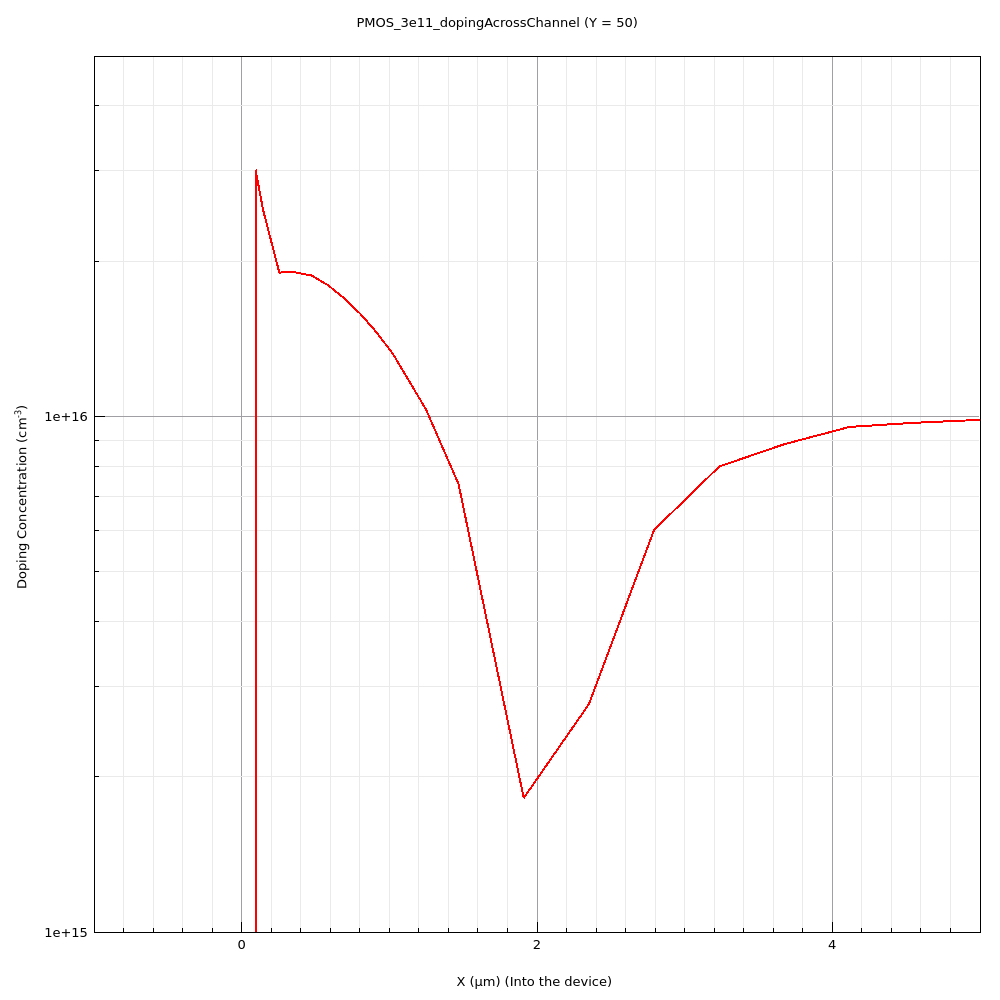
\includegraphics[width=0.5\textwidth]{Figures/PMOS_3e11_dopingAcrossChannel.png}
    \caption{Simulated PMOS dopant concentration across the channel for a VT-adjust dose of $3\times10^{11}~\mathrm{cm^{-2}}$.}
    \label{fig:pmos_cross_section}
\end{figure}

Similarly, for the NMOS, after changing the the dose from 9e11 at/$\text{cm}^2$ to 3e11 at/$\text{cm}^2$, the two doses give almost identical profiles for the across-source plot, the along-device plot, and the cross section except for the across channel doping concentration as well. 

\begin{figure}[H]
    \centering
    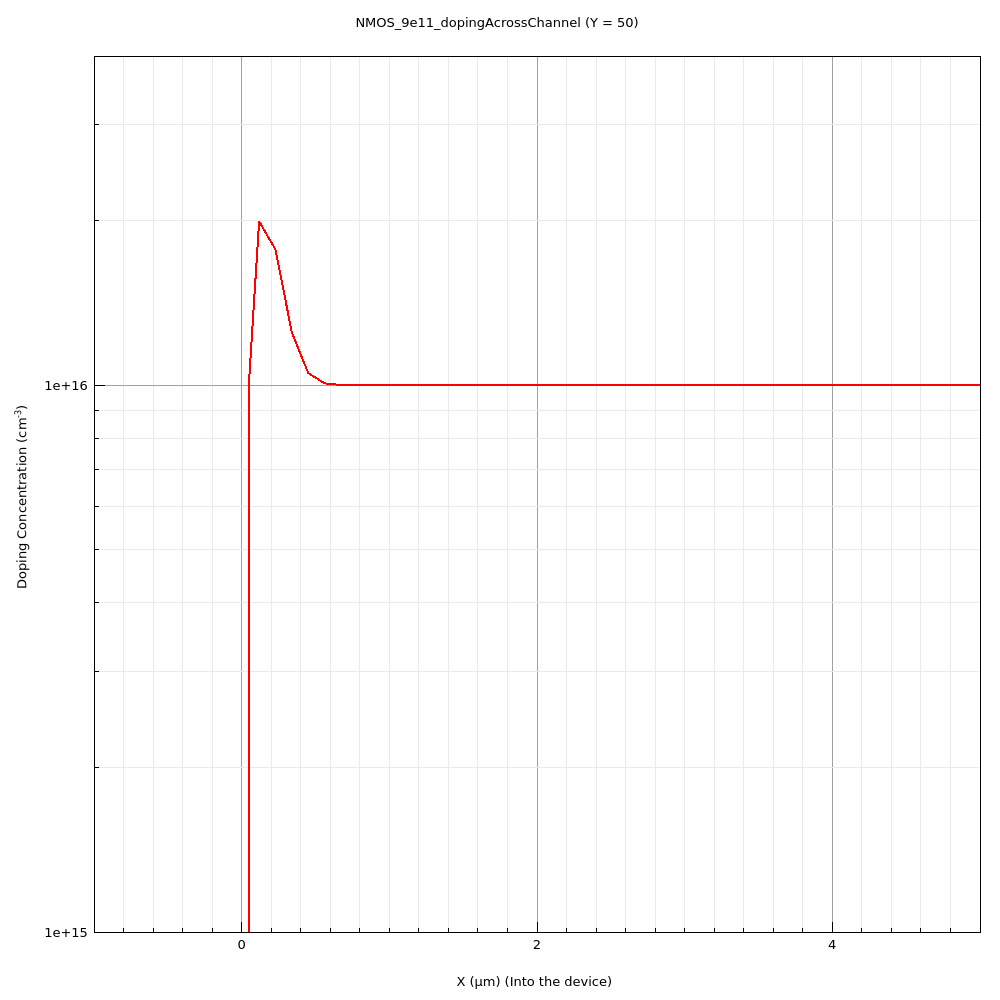
\includegraphics[width=0.5\textwidth]{Figures/NMOS_9e11_dopingAcrossChannel.png}
    \caption{Simulated NMOS dopant concentration across the channel for a VT-adjust dose of $9\times10^{11}~\mathrm{cm^{-2}}$.}
    \label{fig:pmos_cross_section}
\end{figure}

For both devices, the differences between the across channel plots of the two doses are in the near-surface region. More specifically, for the PMOS, the boron $V_\mathrm{T}$-adjust is implanted into the n-type well, where it compensates the phosphorus donors. At $9\times10^{11}\,\mathrm{cm^{-2}}$ the net doping shows a clear compensation notch below the surface, while the notch is absent at the doping concentration of $3\times10^{11}\,\mathrm{cm^{-2}}$. 

And for NMOS, at doping concentration of $9\times10^{11}\,\mathrm{cm^{-2}}$, the boron $V_\mathrm{T}$-adjust raises the net doping to a peak of about $2\times10^{16}\,\mathrm{cm^{-3}}$ within the first $0.2\,\mu\mathrm{m}$, above the $1\times10^{16}\,\mathrm{cm^{-3}}$ substrate background; at $3\times10^{11}\,\mathrm{cm^{-2}}$ the peak is much smaller, about $1.2\times10^{16}\,\mathrm{cm^{-3}}$. Below about $0.5\,\mu\mathrm{m}$ the boron is no longer present and both profiles return to the substrate level. Unlike the PMOS, the $V_\mathrm{T}$-adjust implants boron into a p-type substrate, so the acceptor adds directly to the channel doping instead of compensating a well: the net concentration rises rather than notching, and its excess above the substrate scales with the implanted dose.

For the NMOS the boron is implanted into the p-type substrate, so it adds directly to the channel acceptors, the net doping therefore rises to a peak just below the surface rather than creating a notch, and the peak is larger at $9\times10^{11}\,\mathrm{cm^{-2}}$ than at $3\times10^{11}\,\mathrm{cm^{-2}}$. The height of the peak above this background scales with the implanted dose, below the implanted region the boron is no longer present and both profiles return to the substrate level.


\begin{figure}[H]
    \centering
    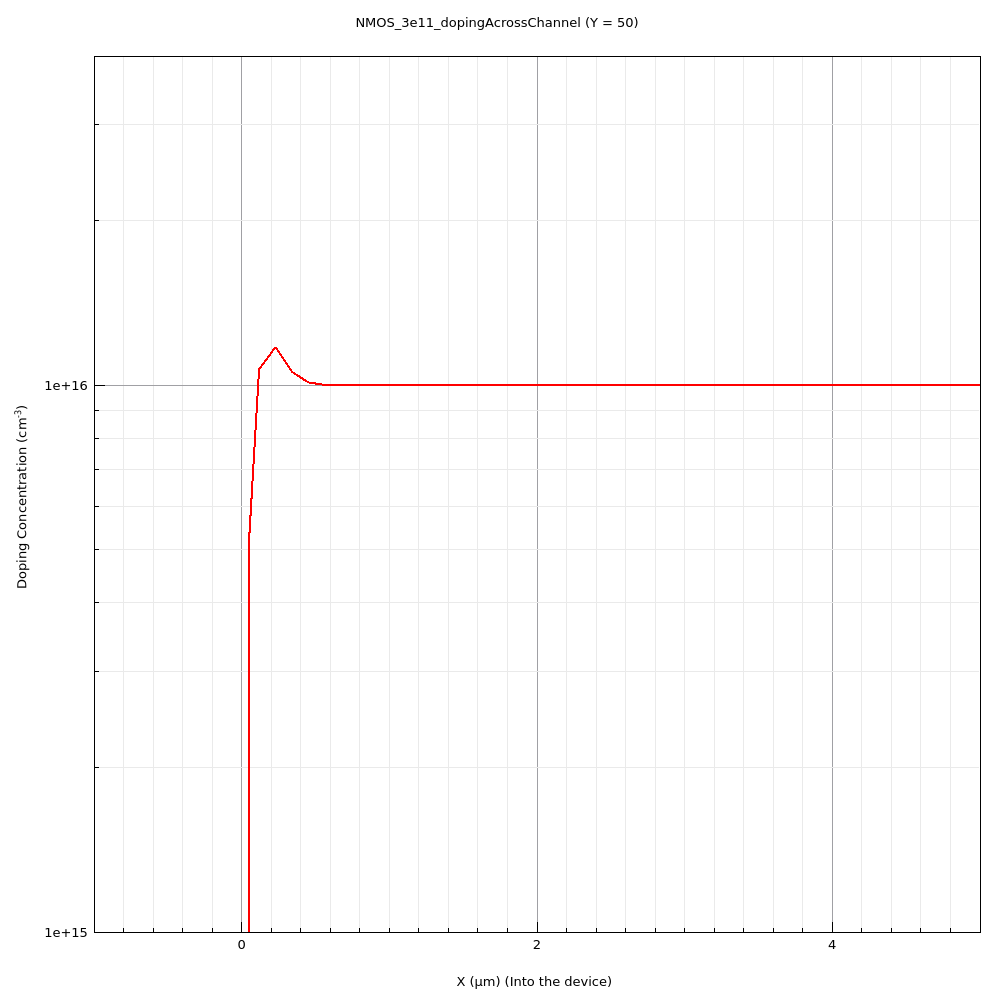
\includegraphics[width=0.5\textwidth]{Figures/NMOS_3e11_dopingAcrossChannel.png}
    \caption{Simulated NMOS dopant concentration across the channel for a VT-adjust dose of $3\times10^{11}~\mathrm{cm^{-2}}$.}
    \label{fig:pmos_cross_section}
\end{figure}

The cause is the boron $V_\mathrm{T}$-adjust, a shallow low-energy implant into the n-type well surface. As an acceptor it partially compensates the phosphorus in the well and lowers the net donor concentration near the surface. The compensation scales with dose, so $9\times10^{11}\,\mathrm{cm^{-2}}$ removes enough net donor to form a local minimum where the boron most closely balances the phosphorus, whereas $3\times10^{11}\,\mathrm{cm^{-2}}$, at one third of the dose, only dents the profile. Below about $0.5\,\mu\mathrm{m}$ the boron is no longer present and the two profiles coincide.



\subsection{Device Simulation - 10 \& 11}


\begin{table}[H]
    \centering
    \caption{Extracted threshold voltage at the three $V_T$-adjust doses
    ($V_D = 0.1$~V for NMOS, $-0.1$~V for PMOS).}
    \label{tab:vt_adjust}
    \begin{tabular}{ l c c c}
        \toprule
        \textbf{VT-adjust dose} & \textbf{$V_T$ (V) for 3E11} & \textbf{$V_T$ (V) for 6E11} & \textbf{$V_T$ (V) for 9E11} \\
        \midrule
        NMOS, $V_{\text{Sub}} = 0\text{ V}$  & 0.77  & 1.03  & 1.26 \\
        NMOS, $V_{\text{Sub}} = -1\text{ V}$ & X     & X     & 2.17 \\
        NMOS, $V_{\text{Sub}} = -2\text{ V}$ & X     & X     & 2.78 \\
        PMOS, $V_{\text{Sub}} = 0\text{ V}$  & -3.23 & -3.00   & -2.81 \\
        \bottomrule
    \end{tabular}
\end{table}




